\documentclass[czech,BP]{thesiskiv}
\usepackage[czech]{babel}
\usepackage{ae}
\usepackage{fancyhdr}
\usepackage{float}
\RequirePackage[nohyperlinks]{acronym}[2005/10/04]
\usepackage{url}
\usepackage{breakurl} 
%\usepackage[breaklinks]{hyperref}
\usepackage{pifont}
\usepackage{graphicx}
\usepackage{listings}
\usepackage{color}
\usepackage{svg}
\usepackage[nottoc,notlot,notlof]{tocbibind}

\usepackage[pdftex]{hyperref}
\hypersetup{colorlinks=true,
  unicode=true,
  linkcolor=black,
  citecolor=black,
  urlcolor=black,
  bookmarksopen=true}

\usepackage[numbers,sort&compress]{natbib}

\setlength\parindent{0pt}

\renewcommand{\lstlistingname}{Výpis kódu}

\lstdefinestyle{customc}{
  belowcaptionskip=1\baselineskip,
  breaklines=true,
  frame=,
  xleftmargin=\parindent,
  language=C,
  showstringspaces=false,
  basicstyle=\footnotesize\ttfamily,
  keywordstyle=\bfseries\color{blue},
  commentstyle=\itshape\color{purple},
  identifierstyle=\color{black},
  stringstyle=\color{orange},
}

\lstdefinestyle{customasm}{
  belowcaptionskip=1\baselineskip,
  frame=,
  xleftmargin=\parindent,
  language=[x86masm]Assembler,
  basicstyle=\footnotesize\ttfamily,
  commentstyle=\itshape\color{black},
  morekeywords={movq,pushq,subq,movl,addl,eax,ebx,ecx,edxs,testl,testb,rbp,rsp,beq,bne}
}

\lstdefinestyle{custombash}{
  belowcaptionskip=1\baselineskip,
  breaklines=true,
  frame=,
  xleftmargin=\parindent,
  language=bash,
  showstringspaces=false,
  basicstyle=\footnotesize\ttfamily,
  keywordstyle=\bfseries\color{blue},
  commentstyle=\itshape\color{purple},
  identifierstyle=\color{black},
  stringstyle=\color{orange},
  morekeywords={make,cmake,git}
}

\lstset{escapechar=@,style=customc}

\author{Martin Úbl}
\declarationmale

\title{Vizualizace dat profilingových nástrojů}


\abstracttexten{The main goal of this paper is to analyze available profiling tools, their output formats, visualization methods of their collected data and to design and implement portable modular tool for such data visualization.

In first chapters, the problem of profiling and collecting performance data is investigated. Next part focuses on analysis of commonly used profiling tools and their output formats, common visualization methods and already available visualization tools.

The second part contains design of modular tool, which would be able to load, analyze and visualize profiling data independently of what profiler was used and which operating system the user runs.

The last part focuses on tool realization, contains implementation details and user documentation.}

\abstracttextcz{Hlavním cílem této práce je analýza dostupných profilingových nástrojů, jejich výstupních formátů, způsobů vizualizace jimi nasbíraných dat a návrh přenositelného modulárního nástroje pro jejich vizualizaci a jeho realizace.

V prvních kapitolách je rozebrána problematika profilingu a způsobů sběru dat. Následuje analýza používaných profilingových nástrojů a formátu jejich výstupu, dále způsobů vizualizace profilingových dat a nástrojů pro vizualizaci, které jsou již dostupné.

V druhé části je obsažen návrh modulárního nástroje, který bude schopen nezávisle na operačním systému a použitém profileru načíst odpovídajícím modulem profilingová data, vnitřně je analyzovat a pomocí výstupního modulu poskytnout jejich vizualizaci.

Poslední část se zabývá realizací nástroje, obsahuje programátorskou a uživatelskou dokumentaci výsledného programu.}

\begin{document}

\pagestyle{fancy}

\newcommand{\tick}{\ding{52}}
\newcommand{\tickcross}{\ding{55}}
\renewcommand{\chaptermark}[1]{\markboth{\textit{#1}}{}}
\renewcommand{\sectionmark}[1]{\markright{\textit{#1}}{}}
\cfoot{\thepage}
\lhead{\leftmark}
\rhead{\rightmark}
\maketitle

\thispagestyle{empty}
\section*{Poděkování}
Rád bych touto cestou poděkoval Ing. Jindřichu Skupovi za odborné vedení a cenné rady v průběhu této práce. Dále patří poděkování panu Jiřímu Jabůrkovi za pomoc při získávání praktických zkušeností v oblasti zkoumané problematiky.


\tableofcontents
\pagestyle{fancy}
\renewcommand{\chaptermark}[1]{\markboth{\textit{#1}}{}}
\renewcommand{\sectionmark}[1]{\markright{\textit{#1}}{}}
\cfoot{\thepage}
\lhead{\leftmark}
\rhead{\rightmark}
\parskip 1em

\newpage

\chapter{Úvod}
Výkon programů, tedy schopnost zpracovat co největší množství dat nebo provést co nejvíce výpočtů za jednotku času, byl vždy velmi důležitým kritériem použitelnosti kteréhokoliv software. Při psaní programového kódu je tedy nutné dbát na vhodnou volbu algoritmu, na způsob zápisu a v krajních případech i na to, jak kompilátor přeloží zapsaný programový kód do binární podoby, případně jak interpret uvnitř odvodí posloupnost operací nutnou k jeho vykonání. Takových informací je ale příliš na to, aby bylo v lidských silách bez pomoci strojové analýzy vyvinout optimální kód - tedy takový, který má prokazatelně největší výkon bez ztráty přesnosti a správnosti výsledku. Proto existují nástroje zvané \uv{profilery}, které analyzují běh programu, výkon jednotlivých částí kódu, případně staticky i kód samotný, aby mohly posléze vygenerovat zprávu o tom, kde program tráví nejvíce času a kde je tedy vhodné provést optimalizaci. Stejně jako profilery nasbíraná data je důležitý způsob jejich prezentování vývojáři, aby mohl optimalizovat tu část programu, která je skutečně zodpovědná za pomalý běh.

Cílem této práce je analyzovat dostupné profilery, jejich výstupní formáty, způsoby, jakým prezentují nasbíraná data uživateli a existující způsoby vizualizace těchto dat obecně, a na základě této analýzy navrhnout a implementovat modulární nástroj, který dovede vizualizovat výstupy různých profilerů v jednotné formě. Modularita bude spočívat v oddělené implementaci jádra aplikace, modulů pro načítání dat z profilerů a modulů výstupních. Dalším požadavkem je přenositelnost mezi běžnými platformami.

Navržený nástroj tedy nebude obstarávat sběr dat, pouze jejich zpracování a vizualizaci standardními způsoby.

\newpage

\chapter{Profiling}

Profiling, někdy nazývaný \emph{výkonnostní analýza}, je způsob vyhledávání míst v programu, která výrazně snižují výkon celé aplikace, popř. celého systému. Takové místo se nazývá \emph{bottleneck} a jeho identifikace nemusí být snadná, stejně jako pozdější řešení. K identifikaci výkonnostních problémů slouží nástroje zvané \emph{profilery}, které se starají o sběr informací z běhu programu a někdy i ze statické analýzy kódu. Tato data pak předají vizualizačnímu nástroji, ať už ve formě souboru nebo datového proudu, a ten je poskytne v lidmi interpretovatelné formě vývojáři.

\section{Výkon}

Bavíme-li se o analýze výkonu programů, je nutné stanovit, co vlastně sledujeme, a co očekáváme, že nám profilery poskytnou. Hlavní veličinou, kterou budeme sledovat, je výkon. V tomto kontextu lze použít fyzikální definici, tedy že výkon je práce vykonaná za jednotku času. U času se můžeme zaobírat pouze jednotkou, tedy za jaký časový úsek budeme práci sledovat - to je ale velmi specifické pro každý případ, a proto se tím nebudeme v obecné rovině zaobírat. Zbývá pouze definovat práci. Tu můžeme v této terminologii popsat například jako počet vykonaných instrukcí, což je exaktní měřítko z hlediska hardware, ale nemusí mít dostatečnou vypovídací hodnotu o skutečné efektivní práci. Proto práci definujeme spíše jako počet vykonaných operací, kde operaci můžeme abstrahovat například na funkční volání. Z toho vyplývá i to, že je nutné důsledně členit programový kód do funkcí (metod, objektů), aby bylo možné tuto metriku vůbec použít.

\section{Bottleneck}

Pojmem \emph{bottleneck} se obecně označuje kterýkoliv element (modul, komponenta, funkce), který způsobuje zpomalení celku (aplikace, stroje). Bottleneck můžeme najít na různých místech, a to nejen v programovém kódu - může například jít o zpoždění při komunikaci přes síť, při zápisu nebo čtení z disku. To jsou takzvané hardwarové bottlenecky, a mají pouze nepřímý vliv na výkon programu samotného. Lze je řešit buď výměnou součástky, nebo jinou fyzickou změnou (výměna kabelu, změna topologie sítě, atd.).

Hlavním bodem zájmu bude ale bottleneck softwarový, tedy ten, co lze optimalizovat pouze změnami v programovém kódu. Nutno dodat, že optimalizace softwarového bottlenecku nemusí nutně znamenat jeho odstranění. Pokud jde například o zápis velkého objemu dat na pevný disk, je samozřejmé, že tato činnost bude trvat delší dobu, a bez optimalizace na úrovni hardware (např. výměna rotačního disku za SSD) se nelze zbavit ani zpoždění při provádění programu. Ve spoustě případů, pokud dokončení zápisu nemusí blokovat běh programu, se ale lze vyhnout čekání, a to například vhodnou paralelizací.

Doba provádění programu bude vždy záviset na hardware. Důležité je proto oddělit problém softwarový od problému hardwarového. Výkonnostní optimalizaci softwarového rázu lze definovat jako takový zásah do programového kódu, který zkrátí dobu provádění daného úseku kódu beze změny jeho výstupu. Použitím abstrakce z předchozí sekce jde o snížení počtu operací, případně o výměnu za méně náročné operace.

Dále se budeme zabývat pouze bottlenecky softwarovými.

\subsection{Typické řešení}

Velmi často vzniká chyba v použití nevhodného algoritmu, a to buď obecně, nebo v závislosti na situaci. Školním případem by byly řadící algoritmy - primitivním způsobem, jak řadit pole čísel, je například \emph{bubble sort}. Jsou ale obecně známy mnohem efektivnější algoritmy řazení pro jakoukoliv množinu čísel. Proto je volba \emph{bubble sortu} obecně nevhodná z hlediska výkonu. Nevhodná volba v závislosti na situaci často spočívá v opomenutí nějakého faktu, který se situací souvisí - například nějaká definovatelná pravidelnost ve vstupních datech. V řadících algoritmech by byla dobrým příkladem seřazená posloupnost na vstupu. Pokud bychom mohli ve většině případů předpokládat seřazenou nebo téměř seřazenou posloupnost, pak není vhodné implementovat algoritmus, který přidává velkou režii v podobě přeskupování již seřazené podposloupnosti (např. \emph{heap sort}), ale je lepší využít takový, který lépe pracuje s téměř seřazenou posloupností (např. \emph{insertion sort} a jeho varianty).

Další typickou příčinou neoptimálního běhu je nevhodné využití datových úložišť obecně. Zpravidla je vhodné mít jako prostředníka mezi pomalým a okamžitým úložištěm nějakou vyrovnávací paměť, takzvanou \emph{cache}. Využitím takovéto paměti odpadá nutnost žádat pomalé úložiště pro každý blok, který nás zajímá. Místo toho lze do cache nahrát mnohem větší množství dat, která jsou například často využívaná, nebo v blízkém okolí aktuálně žádaných dat. Tím je možné minimalizovat přístupovou dobu pro případ opakovaného nebo sekvenčního čtení.

Speciálním případem nepřímo viditelného datového úložiště je cache procesoru, jejíž využití je přímo nutností pro rozumný běh kteréhokoliv programu. Čtení a zápis zde totiž probíhá v několikanásobně kratším čase, než ve standardní operační paměti. To, co se v cache procesoru uchovává je možné v rámci programu ovlivnit například tak, že je respektován princip \emph{lokality} - pokud jsou data uchována v paměti za sebou, a je k ním i tak přistupováno, nevzniká v CPU cache tolik cache-miss\footnote{skutečnost, kdy nebyla nalezena položka v cache procesoru, takže musí být vyzvednuta z pomalejšího úložiště} a provádění programu je podstatně rychlejší.

\section{Kritické optimalizace}

V krajních případech, kdy máme jistotu, že nelze použít lepší algoritmus a nelze lépe optimalizovat přístupy k datovým úložištím, ale stále potřebujeme zvednout výkon, se naskýtá možnost přistoupit k tzv. \emph{kritickým optimalizacím}. Ty spočívají hlavně ve snížení náročnosti na úrovni instrukcí. Velkou část optimalizací na úrovni instrukcí ale dělá sám kompilátor, jelikož se často jedná o typické případy.

Dobrým příkladem kompilátorem obtížně proveditelné optimalizace je minimalizace počtu skoků, které jsou vykonány. Procesory, které implementují pipelining\footnote{způsob paralelního zpracování instrukcí ve vzájemně se nepřekrývajících fázích}, musí totiž při provedení skoku zahodit doposud předzpracované instrukce a začít se zpracováním dalších na novém místě programu. Jelikož ve veškerých moderních programovacích jazycích dochází ke skoku pouze v rámci podmínek a cyklů, budou právě tyto struktury hlavním bodem zájmu při optimalizaci počtu skoků. Co se podmínek týče, lze využít pravděpodobnostní přístup - pokud je pravděpodobné, že podmínka bude splněna ve většině případů, je vhodné zajistit, aby se při splnění podmínky neprováděl skok.

Příklad optimalizace skoku lze vidět v následujících úryvcích kódu. V kódu \ref{branch_1_c} je implementována funkce, která určitým způsobem trasformuje vstupní parametr. Uprostřed funkce je transformace podmíněná, která testuje, zdali se nejedná o krajní případ - funkce \texttt{is\_corner\_case()} bude vracet ve většině případů hodnotu $0$, tedy podmínka splněna nebude. V pseudoassembly kódu \ref{branch_1_asm} lze vidět, že se při nesplnění podmínky provede skok na návěští pod blokem příkazů, co by se provedly při platnosti podmínky. Jelikož podmínka bude splněna ve velmi malém množství případů, bude se naopak ve velkém množství případů provádět skok.

\lstset{escapechar=@,style=customc}
\begin{lstlisting}[caption=Funkce v jazyce C znázorňující nutnost skoku při splněné podmínce, label=branch_1_c]
int testFunction(int value)
{
    value *= 2;
  
    if (is_corner_case(value))
        value += 10;
  
    value *= 2;
  
    return value;
}
\end{lstlisting}

\lstset{escapechar=@,style=customasm}
\begin{lstlisting}[caption=Pseudoassembly verze kódu \ref{branch_1_c}, label=branch_1_asm]
testFunction(VALUE):
    mul     2, VALUE
    call    is_corner_case(VALUE)
    cmp     %eax, 0
    beq     .LBL1
    add     10, VALUE
.LBL1:
    mul     2, VALUE
    ret
\end{lstlisting}

Přepis kódu do pravděpodobnostně optimální podoby by obecně záležel na konkrétní situaci. V tomto případě lze provést invertování podmínky a návrat z funkčního volání o něco dříve při pozitivním scénáři. Jak lze vidět z kódu \ref{branch_2_c}, funkce je o něco delší. Za cenu delšího kódu byl získán takový sled instrukcí, ve kterém je výrazně menší pravděpodobnost skoku.
\\

\lstset{escapechar=@,style=customc}
\begin{lstlisting}[caption=Funkce v jazyce C znázorňující nutnost skoku při splněné podmínce, label=branch_2_c]
int testFunction(int value)
{
    value *= 2;
  
    if (!is_corner_case(value))
    {
        value += 2;
        return value;
    }

    value += 10;
    value *= 2;

    return value;
}
\end{lstlisting}

\lstset{escapechar=@,style=customasm}
\begin{lstlisting}[caption=Pseudoassembly verze kódu \ref{branch_2_c}, label=branch_2_asm]
testFunction(VALUE):
    mul     2, VALUE
    call    is_corner_case(VALUE)
    cmp     %eax, 0
    bne     .LBL1
    add     2, VALUE
    ret
.LBL1:
    add     10, VALUE
    mul     2, VALUE
    ret
\end{lstlisting}

Pokud je možné pravdivost podmínky alespoň s určitou pravděpodobností předpovědět, je vhodné kód přeuspořádat tak, aby byly minimalizovány skokové instrukce, tedy nutnost resetovat pipelining. Tento případ je totiž jedním z mála, který kompilátor nedovede s jistotou optimalizovat - v momentě kompilace totiž nelze strojově určit, zdali je některý scénář splnění podmínky více pravděpodobný. Některé kompilátory kombinované s vývojovým prostředím obsahují možnost tzv. \emph{profile-guided optimalizations}, které právě s pravděpodobností skoků pracují, a výsledný kód na základě nasbíraných dat optimalizují. Pro potřeby této práce je ale nutné znát hlavně fakt, že existují profilery, které četnosti scénářů splnění podmínky počítají a předávají je skrze vizualizační nástroj programátorovi.

Některé kompilátory, například \emph{gcc}, obsahují tzv. \emph{branch prediction built-in} funkci \texttt{\_\_builtin\_expect}, prostřednictvím které lze předat kompilátoru informaci o pravděpodobnosti splnění podmínky. Není tedy nutné kód přeskupovat ručně.



\section{Metody sběru dat}

Způsobů, jakými jsou získávána výkonnostní data, může být více. Mezi hlavními a reálně používanými jsou ale pouze čtyři, které budou popsány v následujících podkapitolách.

\subsection{Vzorkování}\label{subsec:sampling}

Principem vzorkování se rozumí opakované snímkování stavu provádění programu. Každý snímek obsahuje data spojená s funkčním voláním a současným zanořením, hodnotu programového čítače a volitelně i další údaje, jako hodnotu ostatních registrů, informaci o vlákně, které kód vykonává, a další, spíše specifické údaje pro daný profiler.

Vzorky mohou být pořizovány různými způsoby. Starším přístupem je periodické vzorkování čistě na základě času, konkrétně pomocí hardwarového přerušení časovače (IRQ 0). To v první řadě dovolovalo použít vzorkovací mechanismus pro profiling. Nevýhodou byla ale poměrně obtížně definovatelná frekvence, jelikož bylo třeba zvolit přiměřenou granularitu vzorků tak, aby stále poskytovala dostatečně prokazatelná data. 

Podstatné zlepšení přinesl koncept hardwarových výkonnostních čítačů (dále jen HPC), což jsou speciální registry procesoru, jejichž jediným účelem je uchovávat počet vybraných hardwarových událostí. Takovou událostí může být například provedení instrukce, výskyt cache-miss, nutnost pozastavit pipelining kvůli zamezení datovému hazardu (tzv. stalling), a další. Hardwarové výkonnostní čítače jsou ale vždy závislé na konkrétním modelu, popř. řadě procesorů, a ne vždy je k dispozici stejná sada. Problém rozdílnosti těchto sad čítačů řeší modul obecně označovaný jako \emph{perf events} (konkrétně u jádra GNU/Linux označováno jako \emph{Linux Kernel Performance Events Subsystem}) v jádře OS, který poskytuje jednotné rozhraní k používání HPC a přidává další události související například s jádrem OS\cite{perf1}.

Přístup s HPC používá hardwarové přerušení NMI. To je generováno při každém přetečení některého z čítačů, jehož hodnotu sledujeme\cite{perf1}. NMI je specifické v tom, že je vyvoláváno i tehdy, když jsou přerušení momentálně zakázána. Taková situace nastává například přímo při zpracování některých tzv. blokujících přerušení. Je tedy možné provádět profiling i jádra samotného.

\subsection{Instrumentace}

Dalším přístupem je takzvaná \emph{instrumentace}. Ta spočívá ve vložení speciálních profilovacích funkčních volání, která se starají o inkrementaci odpovídajících čítačů volaných a volajících funkcí, a zaznamenání aktuální pozice vykonávání programu na základně hodnoty programového čítače.

Tato volání mohou být buď integrována v čase kompilace přímo kompilátorem (pokud to podporuje), ručně v programovém kódu, nebo dokonce do již zkompilovaného binárního spustitelného souboru.

\subsection{Interpretace}

Podstatně rozdílným přístupem je pojetí zkompilovaného strojového kódu jako intermediate kód\footnote{meziformát určený pro zefektivnění interpretace, lze např. uvést \emph{bytecode} používaný v rámci Java Virtual Machine, nebo \emph{CIL} z prostředí .NET}, který je interpretován nad vlastním virtuálním strojem\cite{grind2}. Tento přístup dovoluje obalit kteroukoliv instrukci jakýmkoliv vlastním kódem, ovšem za cenu výrazného zpomalení běhu.

\subsection{Událostní profiling}

Příbuzným přístupem instrumentaci je událostní profiling. Potenciál tohoto způsobu získávání dat byl využit až v oblasti interpretovaných jazyků, kdy je přímo ve virtiálním stroji, který námi psaný program interpretuje, přítomno sledování určitých událostí, jako je například funkční volání, alokace paměti pro objekt daného typu a další.


\newpage

\chapter{Analýza dostupných nástrojů}

Pro všechny běžné platformy, tedy Windows, Linux a MacOS, existuje poměrně rozsáhlý sortiment profilerů. V této kapitole budou stručně popsány ty, které se řadí mezi nejpoužívanější.

\section{perf}\label{subsec:perf}

Perf je systém pro měření výkonu na operačních systémech založených na jádře GNU/Linux verze 2.6 a vyšší. Využívá metodu vzorkování, a to na základě hardwarových výkonnostních čítačů.

Nutnou podmínkou je tedy podpora v CPU pro výkonnostní čítače, které nás zajímají. Tato podpora byla zaváděna již od modelů procesoru Intel Pentium\cite{perf3} a stala se standardním prvkem pro všechny následující modely nejen firmy Intel. Všechny dnešní procesory architektury x86, x86-64 a dalších tedy tuto podmínku jistě splňují. Dále je nutné provozovat operační systém s implementovanou podporou HPC.

\subsection*{Sběr dat}\label{subsubsec:perf-collect}

Samotný profiling je prováděn pomocí zaznamenávání těchto hardwarově vyvolávaných událostí přes buffer v jádře, a to buď do souboru (\texttt{perf record}) nebo přímo na výstup konzole (např. \texttt{perf top}).

V případě použití \texttt{perf record} jsou zachycené události zapisovány do souboru s implicitním názvem \texttt{perf.data} (lze změnit parametrem). Jedná se o binární soubor obsahující všechny pořízené vzorky. Z takového souboru lze posléze extrahovat různé pohledy - \texttt{perf report} spustí textové rozhraní pro navigaci v rámci seznamu funkcí řazených podle četnosti výskytu zkoumané události, \texttt{perf annotate} sestaví disassembly, ke kterému v případě, že byly do binárního souboru zakompilovány debugovací symboly, připojí i namapovaný zdrojový kód, \texttt{perf diff} pro sestavení rozdílu mezi dvěma reporty, a další.

Ve výstupním souboru je obsažena hlavička a tři sekce. První sekcí je sekce s atributy, obsahující metainformace o vzorcích, druhou sekce se seznamem sledovaných událostí, a třetí sekce se samotnými vzorky nasbíraných za běhu\cite{perf2}.

\subsection*{Výhody a nevýhody}

Velkou výhodou nástroje \emph{perf} je právě ve využívání hardwarové podpory pro zjišťování výkonu, a interfacing s jádrem, které řeší rozdílnost řešení a sady čítačů v CPU samotném. Zkoumaný proces pak není nijak výrazně zpomalen oproti jeho normálnímu běhu, jelikož není nijak měněn instrukční tok programu samotného. Další výhodou je bezesporu sortiment veličin, které je možné zkoumat. Kromě \uv{běžného} zkoumání tráveného času prováděním specifických úseků kódu lze pozorovat i možné příčiny toho, proč je naměřený čas tak dlouhý.

Nevýhoda může být skryta ve výše zmíněném vzorkování. Jelikož je pořízen vzorek v rámci diskrétních časových úseků, může se stát, že nějaký výkyv může uniknout. Vzhledem k tomu, že takové výkyvy většinou trvají mnohem déle, než je perioda vzorkování, není pravděpodobné, že bychom nepozorovali důležitý úsek z hlediska výkonu. Problémy vzorkování v oblasti \emph{perf\_events} lze připodobnit k problémům vzorkování kdekoliv jinde - například vzorkování průběhu matematické funkce s velkými a rychlými výkyvy v průběhu nebo vzorkování průběhu audio signálu při převodu do digitální formy. Další nevýhodou je nutnost mít CPU, který podporuje hardwarové výkonnostní čítače, ale ty jsou v dnešní době standardem ve všech moderních procesorech.




\section{gprof}\label{subsec:gprof}

Gprof je nástroj rozdělený na dvě části - část v kompilátoru a část pro interpretaci dat. V podstatě zaujímá přesně opačné postavení oproti nástroji \emph{perf}. Namísto neinvazivního pozorování procesu na úrovni jádra OS a snímkování událostí z již dostupných zdrojů (HPC) je použita metoda instrumentace. Ta je metodou invazivní, tedy přímo mění instrukční tok při vstupu do bloku instrukcí náležícího každé funkci. Z toho plyne značné zpomalení běhu programu.

Jelikož \emph{gprof} nevyužívá přímo žádnou hardwarovou podporu, jsou prerekvizity čistě softwarové. Pro možnost profilovat tímto nástrojem je nutné mít nainstalovaný kompilátor, který dovede vložit potřebnou posloupnost instrukcí do každé z funkcí. Příkladem takového kompilátoru je \emph{gcc}. Na většině linuxových distribucí je zároveň třeba doinstalovat balík \emph{binutils}, kde je obsažen samotný nástroj pro intepretaci výstupu generovaného vloženými instrukcemi.

Dále je nutné kompilátor instruovat, aby profilovací volání do programu zakompiloval, a to zpravidla pomocí nějakého přepínače. Nástroj \emph{gcc} tato volání integruje při kompilaci s přepínačem \texttt{-pg}.

\subsection*{Sběr dat}\label{subsec:gprofgather}

Jak již bylo zmíněno, v čase kompilace je do instrukčních bloků funkcí zapravena část kódu, která se stará o zaznamenání volání funkce a o měření času stráveného uvnitř funkce v jednom volání. To v případě nástroje \emph{gprof} zaručují dvě funkce - \texttt{mcount()}, která zaznamenává volanou a volající funkci, a \texttt{profil()}, což je systémové volání pro zjištění hodnoty programového čítače a jeho zaznamenání do tabulky v paměti\cite{gprof2}. Toto systémové volání ale nemusí být v jádře implementované, a proto se jeho absence dá do jisté míry substituovat pomocí signálů zasílaných procesu.

Funkce \texttt{mcount()} je zodpovědná za evidenci počtu volání každé funkce. Díky zaznamenání volané i volající funkce v podobě programových čítačů je posléze možné zobrazit celý strom volání, případně vymezit větev, která je z hlediska výkonu kritická.

Funkce \texttt{profil()} nemusí být v daném OS dostupná. V případě, že dostupná je, je typicky volána v určitém časovém intervalu. Každé volání zjistí hodnotu programového čítače a inkrementuje hodnotu počítadla na odpovídající adrese v paměti.

Pokud funkce \texttt{profil()} dostupná není, je využito služeb časovačů v jádře OS k zasílání signálů zkoumanému procesu, kam je dodatečně zakompilována i funkce, která tento signál obstarává. Výsledek zpracování tohoto signálu je v podstatě identický s výsledkem volání funkce \texttt{profil()}, jen v podstatně delším čase a s možným zpožděním kvůli režii přidané na generování a obstarávání signálu.

Po spuštění aplikace zkompilované se zapravením výše uvedených funkcí, je generován soubor s implicitním názvem \texttt{gmon.out} (popř. \texttt{jmenoprogramu.out}), který obsahuje veškerá počítadla zaznamenaná po čas běhu. K jejich interpretaci je možné použít příkaz \texttt{gprof}.

Tento soubor je binární, a kromě hlavičky může obsahovat až tři typy záznamů. Prvním záznamem je histogramový, který je zaznemenán voláním \texttt{profil()}, druhý je takzvaný \emph{call-graph record}, obsahující informaci o funkčním volání zaznamenaným pomocí \texttt{mcount()}. Třetí záznam, tzv. \emph{basic-block record}, může nahradit záznam histogramový, a to v případě, že byl použit \emph{line-by-line} mód, tedy speciální režim získávání dat, který spojuje vzorkovací volání ne s funkcemi, ale s jednotlivými řádky zdrojového kódu. Tato funkcionalita ale již v novějších verzích nástroje \emph{gprof} není obsažena\cite{gprof1}.

Histogramový záznam se vztahuje na určitý rozsah adres, v rámci nichž je ještě výsledná uložená struktura dělená po krocích zahrnujících například rozsah 64 adres. Tento rozsah má společný čítač nazývaný \emph{bin}. Nástroj pak zaznamenává pomocí funkce \texttt{profil()} na jakých adresách se provádění programu vyskytovalo a provede \uv{zaokrouhlení} na nejbližší \emph{bin}, jemuž zvýší jeho čítač. Při analýze je poté provedeno rovnoměrné rozdělení času mezi sousední symboly tak, jak zasahují do příslušných \emph{binů}.

Záznam o funkčním volání, tedy \emph{call-graph record} je zaznamenáván pro každou unikátní dvojici adres z volající a volané funkce, v paměti je mu navyšován čítač funkcí \texttt{mcount()}, kolikrát bylo takové volání provedeno a do výsledného souboru je zapsán pouze počet, kolikrát bylo přesně takové volání provedeno.

\subsection*{Výhody a nevýhody}

Podstatnou výhodou je prakticky žádná přímá závislost na hardware. Jedinou nutnou závislostí zůstává podpora v kompilátoru, který je pro daný systém dostupný. Dalším pozitivem je, že jsou zaznamenány veškerá volání funkcí (krom těch, které jsou kompilátorem inlinovány\footnote{nahrazení volání funkce přímo blokem příkazů, který funkce vykonává} v rámci optimalizací).

Nevýhod je ale podstatně více. První znatelnou nevýhodou je zpomalení běhu programu, což může být fatální pro velké množství případů. Tím odpadá možnost použít \emph{gprof} pro vysokozátěžové systémy, kdy se výkonnostní problém objeví až při dosažení určité meze zátěže. Další podstatnou nevýhodou je nutnost mít program zkompilovaný se zapravenými funkcemi, tedy nelze profiling nijak \uv{vypnout} bez provedení nové kompilace.




\section{OProfile}

Sada nástrojů OProfile je poměrně starým způsobem profilování na systémech založených na GNU/Linux, ale dodnes je udržována a adaptována na nové technologie. Před verzí jádra Linux 2.6 již bylo v rámci OProfile možné využívat podporu hardwarových čítačů, a to použitím specifického driveru, který je v podstatě velmi podobný současné implementaci v rámci Linux Kernel Performance Events subsystému (zmíněného v kapitole \ref{subsec:sampling}). Dále bylo nutné mít zavedený daemon, obstarávající vzorkování hodnot výkonnostních čítačů, který je opět podobný již zmíněnému systému \emph{perf events}.

S implementací subsystému pro hardwarové čítače a integrací \emph{perf events} do samotného jádra OS odpadla nutnost udržování vlastního vývoje jejich substitucí, a bylo možné se soustředit přímo na vývoj samotného profileru.

Nástroj OProfile je nutné stáhnout v podobě zdrojových souborů buď jako archiv, nebo pomocí verzovacího systému \emph{git}. Stažený zdrojový kód je třeba přeložit, je tedy nutné mít nainstalovanou sadu kompilátorů \emph{gcc} a pro potřeby přeložení ještě přítomné závislosti. Další požadavky se mohou lišit podle verze a distribuce operačního systému, jejich přítomnost je kontrolována standardním \texttt{configure} skriptem.

\subsection*{Sběr dat}

Jedná se o vzorkovací profiler, podobně jako nástroj \emph{perf}. V současné době oba tyto profilery dokonce využívají stejný modul v jádře OS.

Výstupem je ale celý adresář \texttt{oprofile\_data}, kde jsou uloženy profilovací vzorky (podadresář \texttt{samples}), logovací výstupy a další věci související s profilingovým sezením. Soubory se vzorky jsou binárního typu a obsahují pouze páry offset:počet, kde offset je programový čítač, a počet je množství vzorků, které bylo na tomto offsetu zaznamenáno. Každý soubor se vzorky může obsahovat vzorky jiného druhu - v závislosti na veličině, kterou sledujeme. To je rozlišeno podle struktury podadresářů a názvu souboru samotného.

Výstup lze interpretovat buď příkazem \texttt{opreport} pro výstup standardní, nebo příkazem \texttt{opgprof}, jehož výstup je přizpůsoben, aby vypadal shodně s výstupem nástroje \emph{gprof}.

\subsection*{Výhody a nevýhody}

Většinu výhod má tento nástroj shodnou s výhodami nástroje \emph{perf}. Oproti němu ale disponuje možností formátovat výstup do stejné podoby jako nástroj \emph{gprof}. Co se podporovaných funkcí týče, dá se říci, že nástroje \emph{OProfile} a \emph{perf} jsou zhruba na stejné úrovni a liší se pouze drobnostmi.

Nevýhody jsou opět poměrně stejné, jen nástroj \emph{OProfile} není obsažen mezi standardními balíčky většiny distribucí a musí se dodatečně překládat a instalovat ručně.




\section{Callgrind a Cachegrind}

Tyto dva nástroje jsou přítomny v jednom velkém balíku vývojářských ladících nástrojů \emph{valgrind} pro systémy unixového typu. Pod jednou sekcí jsou uvedeny proto, že funkcionalita nástroje \emph{cachegrind}, tedy profileru zaměřeným na efektivní využití CPU cache, je v této době ve velké míře již obsažena i v nástroji \emph{callgrind}, který se primárně staral pouze o statistiku volání funkcí a generování stromů volání.

Prvním kritériem pro provozování těchto nástrojů je samozřejmě operační systém - tím může být kterýkoliv z podporovaných OS unixového typu, tedy veškeré distribuce GNU/Linux na většině používaných architektur, Solaris, Android a Darwin (od verze 10.9 i MacOS X)\cite{grind1}. Dále je třeba mít nainstalovaný odpovídající balíček \emph{valgrind}, který obsahuje všechny přidružené nástroje, mezi kterými se objevuje právě i \emph{callgrind} a \emph{cachegrind}.

\subsection*{Sběr dat}

Narozdíl od profilerů z předchozích kapitol, \emph{callgrind} a \emph{cachegrind} (dále pouze souhrnně \emph{callgrind}) používají trochu nezvyklý způsob získávání výkonnostních dat - interpretací. To dovoluje každou instrukci obalit takřka libovolným kódem, který se v případě nástroje \emph{callgrind} stará o počítání funkčních volání, cache-miss nad simulovanou cache, počítání přístupů do paměti a dalších událostí. Skutečnost, že je kód nejprve interpretován, bohužel běh programu značně zpomaluje.

Výsledkem je soubor \texttt{callgrind.out.PID}, kde \texttt{PID} je nahrazeno identifikátorem zkoumaného procesu. Jedná se o soubor, jehož obsahem je textová reprezentace záznamů existujících funkcí a všech funkcí z nich volaných včetně časů (zde označených jako \uv{cena}, jelikož vzhledem ke zpomalení generovaném interpretací nelze porovnávat samotné časy) a pozic, ze kterých byly volány. V hlavičce souboru se navíc nachází výčet všech zkoumaných veličin, které jsou v souboru obsaženy\cite{grind3}.

Výstup lze interpretovat použitím příkazu \texttt{callgrind\_annotate}, který při připojení cesty ke zdrojovým kódům generuje výstup ve formě kódu, kde je ke každé řádce připsán počet výskytů zkoumané události.

\subsection*{Výhody a nevýhody}

Výhodou z hlediska funkcionality je rozhodně způsob, jakým nástroj sbírá data. Je zaručeno, že pokud existuje nějaké slabé místo, a je nástrojem správně interpretováno, tak nezmeškáme jeho průchod, jako tomu mohlo být u nástrojů provádějících vzorkování. Dále je velkou výhodou podpora na poměrně široké škále operačních systémů.

Velkou nevýhodou je ale zpomalení, které je vlivem interpretování kódu generováno. Původně strojový kód totiž nikdy není spuštěn přímo, ale přes další vrstvu, která umožňuje sběr dat. Další nevýhodou je, že je nutné interně určitý sortiment hardwarové funkcionality simulovat, aby došlo k detekci událostí v těchto místech. Typicky jde například o výskyt cache-miss, kdy musí \emph{callgrind} simulovat cache na úrovni programového kódu. Pokud bychom se mohli spoléhat na implementaci s identickým fungováním, pak by o nevýhodu nešlo. Existuje ale velké množství rozdílných architektur, a prakticky každá může danou funkcionalitu implementovat jinak. Proto se musíme spokojit s tím, že je tato simulace sice velmi blízko očekávanému modelu, ale nejde o její identickou implementaci.




\section{DTrace}

DTrace je framework určený obecně pro trasování a sledování veškerých akcí, které samotné jádro nebo zkoumaný program vykonává. Je dostupný pro OS Solaris, MacOS X, FreeBSD a jim příbuzné systémy.

\subsection*{Sběr dat}

Veškerý sběr dat je uskutečněn definicí filtrů a událostí v programovacím jazyce \emph{D}, což je speciální jazyk vyvinutý pro použití v rámci frameworku \emph{DTrace}. Jsme schopni sledovat události jako jsou syscally, čtení nebo zápis na disk, případně využívat již zmíněných hardwarových výkonnostních čítačů. Pro potřeby profilingu můžeme dále například snímkovat zásobník specifického procesu na určité frekvenci příkazem

\lstset{escapechar=@,style=custombash}
\begin{lstlisting}
dtrace -n 'profile-99 /pid == 189 && arg1/ { @[ustack()] = count(); }'
\end{lstlisting}

Výstupem je pouze textová reprezentace zaznamenaných hodnot na konzoli nebo do souboru.

\subsection*{Výhody a nevýhody}

Výhodou je bezesporu to, že je \emph{DTrace} velmi obecným a dynamickým nástrojem, který oplývá vlastním programovacím jazykem. Můžeme si tak snáze přizpůsobit průběh trasování specifickým potřebám bez nutnosti použití externích nástrojů. Také je možné sledovat širokou škálu událostí, systémových veličin a používat hardwarovou podporu sledování výkonu.

Nevýhodou je hlavně složitost. Bez znalosti používaného jazyka nelze využívat jeho potenciál v plné míře. Spousty uživatelů \emph{DTrace} se proto soustředí pouze na používání skriptů, které již byly v minulosti napsány a používány za specifickým účelem.




\section{Visual Studio Performance Profiling}

V rámci vývojového prostředí Microsoft Visual Studio je od verze 2010 přitomen i nástroj pro sledování výkonu - Visual Studio Performance Profiling (dále jen \emph{VSPerf}). Principielně nabízí možnost měřit výkon využitím hardwarových výkonnostních čítačů a snímkováním zásobníku (mód \uv{CPU Sampling}, ekvivalentní k nástroji \emph{perf}), dále pomocí zakompilovaného kódu a počítadel zkoumat určité veličiny zblízka (mód \uv{Instrumentation}, principem ekvivalentní k nástroji \emph{gprof}), pokud je aplikace psána pro .NET Framework, pak poskytuje možnost sledovat práci s pamětí, identifikovat místa s největší četností požadavků o alokaci a sledovat funkci garbagge collectoru. Také je přítomen mód pro detekování synchronizačních problémů, které vyúsťují k podstatnému snížení výkonu (příliš dlouhá kritická sekce, apod.).

Pro používání těchto nástrojů je nutné mít nainstalován OS MS Windows ve verzi XP nebo novější. Dále je třeba stáhnout a nainstalovat Microsoft Visual Studio alespoň ve vezi 2010.

\subsection*{Sběr dat}

Metody sběru dat byly popsány již v kapitolách \ref{subsec:perf} (CPU sampling) a \ref{subsec:gprof} (Instrumentation). Metoda použitá ve sledování správy paměti v .NET aplikacích se principielně blíží nástrojům sady \emph{valgrind}, jen s tím rozdílem, že se v tomto případě jedná o interpretovaný intermediate kód i bez použití dalšího nástroje.

Výstupem je soubor se sesbíranými daty, určený k prohlížení v rámci nástroje Visual Studio. Ten dovede vizualizovat interaktivní strom volání, vyhodnotit tzv. \uv{Hot Path}, tedy výkonnostně kritickou větev stromu volání, vyhodnotit funkce, které vykonáváním vlastního kódu (tedy bez volání ostatních funkcí) zabíraly největší procento času a další, spíše doplňkové funkce. Formát výstupního souboru má uzavřenou specifikaci. Možné je ale provést export zformátovaných dat do formátů CSV nebo XML, které obsahují potřebné údaje pro zrekonstruování pohledů. Tento export je ale ztrátový, a tak neumožňuje na základě obsažených dat vytvořit pohledy jiného charakteru.

\subsection*{Výhody a nevýhody}

Mezi výhody patří zejména integrace do jednoho z nejpoužívanějších IDE na OS MS Windows. Tím, že je implementace obstarána přímo na úrovni tohoto prostředí, je zaručena maximální kompatibilita, a lze přímo využívat funkcí prostředí. Další výhodou je možnost využít různé přístupy ke sběru dat v závislosti na tom, co zkoumáme, a to beze změny způsobu vizualizace.

Nevýhodou je nemožnost použít profilingový nástroj bez nutnosti mít nainstalované IDE. Je sice možné spouštět profiling z příkazové řádky, ale stále je potřeba mít k dispozici zbytek vývojového prostředí. To i v minimální nutné instalaci zabírá několik stovek megabajtů až jednotek gigabajtů v závislosti na verzi a edici.




\section{Very Sleepy}

Very Sleepy je jednoduchý profiler pro OS Windows, který vzniknul jako klon staršího, dnes již nevyvíjeného profileru Sleepy. Jedná se o neinvazivní profiler, který podobně jako ostatní profilery z této kategorie pouze sleduje v pravidelných intervalech zásobník zkoumaného procesu (popř. analogicky zásobníky všech vláken daného procesu) a na základě generovaného stromu volání tvoří statistiku.

Pro používání je nutné mít nainstalován OS Windows verze XP a vyšší. Poté stačí mít pouze stažený profiler \emph{Very Sleepy}, jehož balíček obsahuje vše potřebné.

\subsection*{Sběr dat}

Jak bylo uvedeno, jedná se o neinvazivní profiler, který ve velmi krátkých pravidelných intervalech vzorkuje zásobník, extrahuje údaje o funkčním volání a inkrementuje čítače u funkcí, které se v tomto vzorku nachází. Zároveň na základě programového čítače identifikuje i instrukci, u které také provede inkrementaci čítače. Metrikou je zde tedy \uv{počet výskytů}, který by měl být snadno převeditelný na čas, který je v dané funkci tráven.

Výstupem je primárně pouze vizualizace v podobě přehledu volaných funkcí a procenty času tráveného jejich prováděním. Celé profilingové sezení je také možné uložit do souboru binárního typu, případně exportovat do formátu CSV.

\subsection*{Výhody a nevýhody}

Výhodou je jistě to, že jde o velmi malý nástroj. Není třeba žádných dodatečných knihoven, ani velkých balíků závislostí.

Oproti zkoumaným profilerům má ale značně více nevýhod. Jelikož jde opět o profiler, který provádí vzorkování, objevuje se zde znovu možnost, že nějakou skutečnost přehlédne. Také má implementován pouze základní pohled, jehož obsahem jsou pouze procenta tráveného času v jednotlivých funkcích. Mimo to obsahuje poměrně velké množství nedodělaných, nedoladěných funkcí, což má za příčinu jistou nestabilitu.

Pro profiling menších aplikací za účelem získat orientační přehled o možných slabých místech se ale hodit může.





\section{RotateRight Zoom}

Tato sada nástrojů je určena pro operační systémy založené na GNU/Linux a MacOS X. Profiler funguje na již popsaném principu vzorkování, obdobně jako třeba nástroje \emph{perf} nebo \emph{OProfile}. Má ale několik vybraných odlišností v doplňových funkcích.

Od ostatních výše uvedených nástrojů se liší hlavně tím, že nejde pouze o profiler, ale celou sadu nástrojů, obsahující například profiling server, který dovoluje přes síť vzdáleně zpřístupnit rozhraní k profilování. Není tedy nutné mít pro pokročilou vizualizaci výsledků nainstalované grafické prostředí, což je výhodou zejména při profilování na vzdálených serverech, kde by bylo jinak grafické prostředí zbytečné. Také obsahuje statický analyzér kódu, takže je schopen do jisté míry i bez profilování určit potenciální slabá místa.

\section{Shrnutí}

Analyzované nástroje implementují tři různé způsoby sběru výkonnostních dat (shrnuto v tabulce \ref{table:profmethods}). Prvním je vzorkování, tedy neinvazivní snímkování zásobníku a registrů, které sice výrazně nezpomaluje běh zkoumaného programu, ale nemusí poskytovat stoprocentně přesná data. Druhým je instrumentace, čili zakompilování diagnostických volání přímo do programu, což zpomaluje běh podstatně více, ale poskytuje to často velmi přesný přehled o provádění každého funkčního volání - u těchto nástrojů musíme operace konkretizovat na volání funkcí (metod). Třetím způsobem je interpretování spustitelného souboru \uv{virtuálním strojem}, kde můžeme zkoumat prakticky libovolnou veličinu, ale běh programu je zpomalen za produkčně únosnou mez.

Výrazně se tedy liší situace, kdy je který nástroj vhodné použít. Nemusí však jít pouze o rozdílné druhy software - můžeme zkoumat stejný software, jen z jiného úhlu pohledu. Z tohoto důvodu je třeba, aby bylo možné nasbírané informace vizualizovat ideálně v jednotné formě. To by mimo jiné dovolilo vývojáři porovnat výsledky nad normalizovaným pohledem, a tedy by mohlo vést ke spolehlivějšímu odhalení bottlenecku. V případě všech headless\footnote{systémy bez nainstalovaného grafického prostředí, často pouze se vzdáleným terminálovým přístupem} systémů může být problémem i to, že pokud požadujeme pokročilejší vizualizační techniky, je nutné mít nainstalované grafické prostředí, což není na většině serverů obvyklé. Mimo to lze sice vygenerovat nějaké statické výstupy (např. ve formátu SVG), ale ty se často liší od různých nástrojů - tedy buď úplně chybí, nebo nemají jednotnou formu.

Dalším zřejmým problémem je dostupnost napříč různými operačními systémy (znázorněno v tabulce \ref{table:profoss}). Tento problém sice nelze efektivně vyřešit, ale je možné poskytnout takovou vizualizaci dat, která na operačním systému závislá nebude.

Těmito problémy se budou zaobírat následující kapitoly - bude navržen přenositelný nástroj, který bude schopen načíst výstupní formáty profilerů, analyzovat je, a pomocí známých vizualizačních technik poskytnout ucelený pohled, jehož dostupnost nebude podmíněna platformou. Pro potřeby této práce bude nástroj analyzovat pouze výstupy nejpoužívanějších nástrojů pod GNU/Linux, tedy nástroje \emph{perf} a \emph{gprof}. Bude ale navržen tak, aby bylo možné kdykoliv rozšířit podporu i pro jiný formát pouze připojením modulu.

\begin{table}[h]
    \begin{center}
        \def\arraystretch{1.2}
        \begin{tabular}{ c || c | c | c }
              ~ & vzorkování & instrumentace & interpretace \\
            \hline
            \hline
              perf & \tick & \tick & \tickcross \\
              gprof & \tickcross & \tick & \tickcross \\
              OProfile & \tick & \tickcross & \tickcross \\
              Callgrind & \tickcross & \tickcross & \tick \\
              DTrace & \tick & \tickcross & \tickcross \\
              VSPerf & \tick & \tick & \tickcross \\
              Very Sleepy & \tick & \tickcross & \tickcross \\
              RotateRight Zoom & \tick & \tickcross & \tickcross \\
            \end{tabular}
        \caption{Tabulka způsobu sběru dat}\label{table:profmethods}
    \end{center}
\end{table}

\begin{table}[h]
    \begin{center}
        \def\arraystretch{1.2}
        \begin{tabular}{ c || c | c | c }
              ~ & Windows & GNU/Linux & MacOS \\
            \hline
            \hline
              perf & \tickcross & \tick & \tickcross \\
              gprof & \tickcross & \tick & \tick \\
              OProfile & \tickcross & \tick & \tickcross \\
              Callgrind & \tickcross & \tick & \tick \\
              DTrace & \tickcross & \tickcross & \tick \\
              VSPerf & \tick & \tickcross & \tickcross \\
              Very Sleepy & \tick & \tickcross & \tickcross \\
              RotateRight Zoom & \tickcross  & \tick & \tick \\
            \end{tabular}
        \caption{Tabulka podpory profilingových nástrojů na nejpoužívanějších platformách}\label{table:profoss}
    \end{center}
\end{table}







\newpage

\chapter{Analýza vizualizačních technik}

Shromážděná data profilingovými nástroji je nutné převést do formy, které bude vývojář rozumět, a bude na základě ní schopný provést odpovídající změny v kódu. Jelikož jsme použili abstrakci operace na funkční volání, budou zejména konkrétní funkce subjektem zkoumání.

Před analyzováním jednotlivých pohledů je třeba nadefinovat dva pojmy - \emph{inkluzivní čas} a \emph{exkluzivní čas}. Čas trávený ve funkci je totiž nutné rozlišit na část, která byla strávena pouze v rámci instrukčního toku dané funkce, a část, která byla strávena prováděním funkcí z této funkce volaných. Lze snadno vyvodit, že \emph{exkluzivní čas} udává tu část, která byla trávena pouze prováděním zkoumané funkce (exkludovali jsme čas volaných funkcí), a \emph{inkluzivní čas} udává celkový čas včetně času stráveném ve volaných funkcích.

\section{Flat view}

Flat view, jinak nazývaný i \uv{function view}, je prostý seznam funkcí s četností jejich volání, inkluzivním a exkluzivním časem (popř. vzorky). Jedná se o nejjednodušší pohled, který lze vygenerovat, a často je dostačující pro detekci možných bottlenecků. Postrádá ale kontext. Například nelze vydedukovat poměr počtu volání a náročnosti funkce. Nelze tedy přímo zjistit, zdali je třeba optimalizovat počet volání, nebo tělo funkce.

Z tohoto pohledu tedy lze vydedukovat pouze základní problémy a hodí se pouze pro jednoduché programy bez většího množství funkcí. V takových případech lze často kontext vypustit, jelikož je zřejmé, odkud je která funkce volaná.

\begin{figure}[h]
    \centering
    \includegraphics[interpolate,width=1.0\textwidth]{img/prof_flatview.png}
    \caption{Flat view generovaný nástrojem VSPerf}
    \label{obr:flatview}
\end{figure}

\newpage

\section{Hierarchical view}

Hierarchický pohled (také \emph{call tree}, \emph{strom volání}) přidává kontext do předchozího případu. Konkrétně jde o dedukování, která funkce volala kterou, tedy je možné snáze identifikovat možný výkonnostní problém, pokud není přímo ve volané funkci, ale v kontextu okolo.

Tento pohled výrazně rozšiřuje množinu identifikovatelných problémů. Příkladem problému, který odhalí tento pohled navíc oproti \emph{flat view}, je například ten, kdy máme poměrně náročnou funkci, která je volaná z mnoha míst v celém programu. Pokud je ale někde chybně volána častěji, než je nezbytně nutné, bude velké procento volání (popř. vzorků, tráveného času) zvýrazňovat místo problému.

\begin{figure}[h]
    \centering
    \includegraphics[interpolate,width=1.0\textwidth]{img/prof_calltree.png}
    \caption{Hierarchical view generovaný nástrojem VSPerf}
    \label{obr:hieview}
\end{figure}

\section{Graph view}

Grafový pohled je grafickým vylepšením pohledu hierarchického. Výhodou je možnost vidět všechny vazby naráz, bez duplikace jednotlivých funkcí v několika větvích stromu.

\begin{figure}[H]
    \centering
    \includegraphics[interpolate,width=0.5\textwidth]{img/prof_graph.png}
    \caption{Graph view s vyznačenou \emph{hot path}, Zdroj: \url{http://claudiovz.github.io/scipy-lecture-notes-ES/advanced/optimizing/index.html} }
    \label{obr:gview}
\end{figure}

V hierarchickém pohledu totiž mohla nastat situace, kdy se v celém stromu jedna funkce vyskytuje na více místech, a to tehdy, pokud je volána z několika jiných funkcí. V grafovém pohledu jsou všechny duplikáty sloučeny do jednoho uzlu a z uzlů představujících volající funkce jsou do něj vedeny hrany.

\section{Object-method view}

V podstatě se jedná o \emph{flat view}, ovšem v modifikaci pro programy psané v objektově orientovaném jazyce. Položky seznamu (zde metody), jsou sdruženy do skupin podle náležitosti třídě. Pokud je program správně dekomponován, lze pomocí tohoto pohledu identifikovat třídu, jejíž metody představují časově nejnáročnější operace.

\begin{figure}[H]
    \centering
    \includegraphics[interpolate,width=0.8\textwidth]{img/prof_objectview.png}
    \caption{Object-method view, Zdroj: \url{http://kprof.sourceforge.net/} }
    \label{obr:objview}
\end{figure}

Výhoda tohoto pohledu může spočívat například v použití pro týmově vyvíjený produkt, kde každou komponentu měl na starosti jiný vývojář. Lze tedy snadno identifikovat osobu zodpovědnou za pomalý běh. Další vlastnosti tento pohled přebírá od \emph{flat view}.

\section{Flame graph}

Tento pohled lze snadno generovat z pohledu hierarchického. Ve své podstatě jde pouze o expandovaný hierarchický pohled, který je uspořádán odspoda (kořen) nahoru (listy). Značnou výhodou je škálování jednotlivých položek podle procentuálních hodnot zkoumané veličiny - tráveného času (zde inkluzivního). Kořen zaujímá $100\%$ šířky grafu, a veškeré volané funkce jsou o úroveň výše, škálované relativně vůči celkovému exkluzivnímu času volající funkce a jsou vyneseny tak, aby zaujímaly přesně takovou procentuální šířku.

Tento druh vizualizace lze považovat za přínosný zejména z toho důvodu, že znáznorňuje poměrný strávený čas vůči všem ostatním volaným funkcím. Tyto poměry nemusí být z hierarchického pohledu vidět. Také tento pohled významně redukuje množství dat a efektivně eliminuje nevýznamné položky - ty mají ve výsledném grafu minimální šířku.

Takový graf ale vzhledem ke své obsáhlosti musí být buď dostatečně velký, nebo interaktivní. Interaktivitu si můžeme představit například možností rozkliknout funkci, která je pro nás zajímavá - poté se změní poměry šířek, vybraná funkce tvoří výchozí bod se $100\%$ šířkou a všechny ostatní jí volané funkce škálujou podle ní.

\begin{figure}[h]
    \centering
    \includegraphics[interpolate,width=1.0\textwidth]{img/prof_flame.png}
    \caption{Flame graph, Zdroj: \url{http://www.brendangregg.com/FlameGraphs/cpuflamegraphs.html} }
    \label{obr:flamegr}
\end{figure}

\subsection{Detailed graph}

Variací \emph{flame graph} pohledu je tzv. detailní pohled. Ten pouze zužuje celkový pohled na výběr třech po sobě jdoucích úrovní. U takového pohledu je tedy nutná jistá interaktivita, která spočívá v možnosti procházet jednotlivé úrovně klikáním. Dále může být připojen výpis programového kódu se zvýrazněnými částmi, které jsou z hlediska výkonu významné.

\begin{figure}[h]
    \centering
    \includegraphics[interpolate,width=1.0\textwidth]{img/prof_detailgraph.png}
    \caption{Detailed view generovaný nástrojem VSPerf}
    \label{obr:detailview}
\end{figure}

\section {Heat maps}

Heat mapy nejsou v současné době příliš rozšířenou technikou vizualizace profilingových dat, ale je možné je pro určité body zájmu aplikovat. Oproti předchozím způsobům dovoluje zobrazovat do určité míry i trojrozměrná data. Vodorovná osa znázorňuje tok času, svislá osa zkoumané body zájmu, v případě profilingu jde o funkce (metody). Osa času je často diskretizovaná na časové úseky větší, než je snímkovací perioda, jelikož je nutné za tento interval nasbírat takový počet výskytů zkoumaného jevu (programový čítač ukazuje na instrukci z instrukčního toku funkce), aby bylo možné rozlišit významnost.

\begin{figure}[h]
    \centering
    \includegraphics[interpolate,width=1.0\textwidth]{img/prof_histogram.png}
    \caption{Histogram četností dob odezvy pevného disku při čtení a zápisu, Zdroj: \url{http://www.brendangregg.com/HeatMaps/latency.html}}
    \label{obr:heathistoview}
\end{figure}

Na obrázku \ref{obr:heatview} je vidět heat mapa odezvy pevného disku, což je momentálně jeden z hlavních případů použití této techniky. Vodorovná časová osa je rozdělena na diskrétní úseky po 1 vteřině a v rámci tohoto časového úseku bylo provedeno několik stovek čtení. Po uplynulé vteřině byl z časů odezvy vytvořen histogram četností (obrázek \ref{obr:heathistoview}), výšky sloupců byly převedeny na intenzitu barvy, a do výsledného grafu byl takto obarvený sloupec vložen ve vertikálním směru.

\begin{figure}[h]
    \centering
    \includegraphics[interpolate,width=0.8\textwidth]{img/prof_heatmap.png}
    \caption{Heat map, Zdroj: \url{http://www.brendangregg.com/HeatMaps/latency.html}}
    \label{obr:heatview}
\end{figure}

Výhodou takového grafu může být zejména viditelnost tendence. Na základě takto viditelných dat je možné posléze odhadovat, jak se bude program chovat při násobně větší zátěži. Určité aplikace totiž nedovolují provádět profiling při vysoké zátěži a to zejména kvůli zpomalení, které profilery způsobují. Příkladem mohou být veškeré služby, u kterých je žádoucí minimální odezva - kromě realtime systémů lze uvést například herní servery pro masově hrané hry, kde může vyšší odezva znamenat zhoršení herního zážitku.

\section{Shrnutí}

Způsobů vizualizace existuje poměrně velké množství, z velké části jde ale o modifikaci nebo kombinaci způsobů výše uvedených. Každý pohled zvýrazňuje trochu jinou informaci, přičemž záleží vždy na konkrétním případu užití, jak je interpretována. Proto je důležité mít k dispozici co možná nejširší škálu různých pohledů.

Také je vhodné řešit, jakým způsobem, tedy pomocí jakého \uv{média} bude výsledek předán vývojáři. Velká část nástrojů poskytuje výsledky v textové formě, čili snadno zobrazitelné kteroukoliv konzolí. Některé nástroje obsahují vlastní GUI, které je ovšem často závislé na platformě nebo grafickém prostředí. Dále malá skupina nástrojů poskytuje možnost exportovat výsledek do nějakého známého obrazového formátu - typicky PNG nebo SVG.

V rámci této práce bude realizován výstup do pohledů \emph{flat view}, \emph{hierarchical view}, \emph{flame graph}, a budou prozkoumány možnosti \emph{heat map} pohledu pro potřeby profilingu. Dále bude zahrnuta vizualizace do formy webové prezentace, tedy za použití technologií HTML, CSS a Javascript. Zároveň bude dodržena podobná modularita jako u vstupů, tedy bude možné kdykoliv přidat další \uv{médium} jen přidáním modulu.


\newpage

\chapter{Dostupné nástroje pro vizualizaci}

Vizualizačních nástrojů existuje také poměrně velké množství. Kritériem výběru by byl určitě podporovaný profiler, jehož data lze nástrojem zpracovávat, dále určitě závislost na platformě, podporované vizualizační techniky a případně další kritéria, jako je například interaktivita.

\section{Visual Studio Performance Profiling}

VSPerf je kombinovaným řešením, tedy obsahuje i vizualizaci nasbíraných dat. Jedná se o uzavřené řešení, podporován je pouze formát samotného profileru z této sady, z čehož opět vyplývá i závislost na prostředí MS Visual Studio a OS MS Windows. Data lze zobrazit pomocí \emph{flat view}, \emph{hierarchical view}, \emph{detailed graph} a dalších, nepříliš významných technik.

Nástroj poskytuje pouze GUI se všemi pohledy, tedy nelze generovat žádná obrazová data, ani jiný přenositelný formát výstupu.

\section{KCachegrind}

Pro nástroje Callgrind a OProfile lze použít vizualizační prostředí KCachegrind. Jedná se o grafické prostředí, které ke svému běhu potřebuje OS GNU/Linux a grafické prostředí KDE, a je schopné vizualizovat data v pohledech \emph{flat view}, \emph{hierarchical view}, \emph{graph view} a něčem, co připomíná \emph{flame graph}.

Kromě GUI umožňuje KCachegrind navíc exportovat grafy do vektorových formátů.

\section{KProf}

Tento nástroj je velmi podobný nástroji předchozímu, jen dovede zpracovávat data nástroje \emph{gprof} a jemu podobných. Také se jedná o grafické prostředí vyžadující OS GNU/Linux a grafické prostředí KDE. Implementuje pohledy \emph{flat view}, \emph{hierarchical view}, \emph{graph view} a \emph{object-method view}. Jedná se o podstatně jednodušší prostředí, než kterékoliv výše uvedné, ale pohledy nejsou ochuzeny o nic podstatného.

Tento nástroj poskytuje pouze GUI, opět tedy není přítomna žádná možnost, jak zpracovaná data přenést na jinou platformu.

\section{GProf2dot}

Poměrně cenným nástrojem v oblasti vizualizace profilingových dat je \emph{gprof2dot}. Původně dokázal zpracovat pouze výstupy nástroje \emph{gprof}, postupně byla podpora rozšířena na širokou škálu profilerů zahrnujících \emph{perf}, \emph{OProfile}, \emph{callgrind}, i například \emph{Very Sleepy}. Jelikož se jedná o skript psaný v jazyce Python, jeho přenositelnost je podmíněná existencí interpretu pro danou platformu, a také několika málo závislostmi. Oficiálně jsou podporovány OS MS Windows a GNU/Linux. Výstupem je vždy pouze \emph{graph view}, který lze poměrně ve velké míře přizpůsobovat.

Nástroj sice neposkytuje GUI, zato výstupem je obrázek v rastrovém nebo vektorovém formátu.

\section{RotateRight Zoom}

Podobně jako VSProf je i RotateRight Zoom kombinovaným uzavřeným řešením. Dokáže tedy zpracovávat pouze data nashromážděná vlastním profilerem. Oproti předchozím nástrojům má tu výhodu, že lze vizualizovat data na kterékoliv z nejpoužívanějších platforem. Ačkoliv není podporován profiling na OS MS Windows, existuje pro něj grafické rozhraní, které dovoluje zobrazovat data z profilingu probíhajícího na vzdáleném serveru. Kromě \emph{flat view} a \emph{hierarchical view} implementuje i pohled \emph{timeline}, tedy časové osy.

Nástroj obsahuje GUI a zároveň je možné exportovat data do textového formátu.

\section{Shrnutí}

Dostupné nástroje často buď neposkytují přenositelnost výstupu, neobsahují potřebné pohledy, nebo nepodporují širší škálu profilerů.

Obsahem následující kapitoly bude návrh takového nástroje, který poskytne vysokou přenositelnost výstupu, velký výběr pohledů na profilingová data a zároveň zaručenou podporu pro velké množství profilerů, resp. jejich výstupních formátů. V rámci této práce bude realizováno jádro takového nástroje, a implementace pouze vybraných vstupních a výstupních modulů.



\newpage

\chapter{Návrh nástroje}

Účelem nástroje bude načítat profilingová data z výstupních souborů známých profilerů, analyzovat je a následně vizualizovat pomocí vybraného výstupního modulu. Jedním z hlavních požadavků je i modularita nástroje, která bude spočívat ve členění na tři hlavní skupiny modulů, jak je znázorněno na obrázku \ref{obr:systemmodules}. První částí je pevný základ, tedy samotná spustitelná část. Ta bude přejímat požadavky od uživatele, vybírat vstupní modul, analyzovat data a předávat je výstupnímu modulu. Druhou skupinou jsou vstupní moduly - pro každý formát bude existovat právě jeden vstupní modul. Tyto moduly se budou starat o načtení dat, transformaci do jednotné formy a předání zpět do jádra nástroje. Poslední skupinou jsou výstupní moduly, kterým jsou předána analyzovaná data opět v jednotné formě. Tyto moduly na základě vstupních parametrů od uživatele poskytnou požadovaný výstup.

Aplikace bude pouze konzolová. Tím je odbourána závislost na jakémkoliv grafickém prostředí.

\begin{figure}[h]
    \centering
    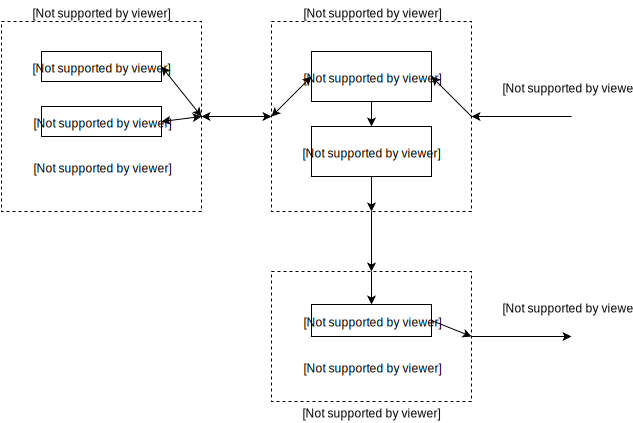
\includegraphics[interpolate,width=1.0\textwidth]{img/system_diagr.png}
    \caption{Architektura nástroje, rozdělení do třech hlavních skupin modulů}
    \label{obr:systemmodules}
\end{figure}

\section{Základ systému}

Tato skupina modulů bude představovat spustitelný program. Moduly základu budou tedy pevně svázány po čase kompilace, tedy nebudou fyzicky oddělitelné. To z důvodu, že je nutné mezi nimi zajistit maximální kompatibilitu, kterou lze do jisté míry zaručit při sestavení.

\subsection{Jádro}

Hlavním úkolem jádra bude obstarávat propojení všech modulů, které budou zapojeny do procesu zpracování vstupů, analýzy a následně formátování výstupu. Samotné jádro bude mít znalost pouze rozhraní se vstupními moduly a s analyzérem, kterému předá zpracovaná data ze vstupních modulů.

Jádro bude představovat i vstupní bod programu, tedy bude přejímat parametry příkazové řádky a na základě nich vybírat příslušné moduly a parametry vizualizace. Také se bude starat o logovací výstupy, které bude možné tisknout buď do konzole, nebo přesměrovat do souboru.

\subsection{Analyzér}

Tento modul bude na vstupu očekávat dostupná profilingová data v normalizovaném formátu, která bude analyzovat a tvořit z nich datové struktury pro jednotlivé pohledy. Bude tedy zodpovědný za první část sestavení pohledů. Druhá část bude implementována až v samotném výstupním modulu, který pouze přečte naformátované datové struktury a vytvoří z nich konkrétní pohled.

Analyzér nesmí předpokládat existenci veškerých dat, jelikož ne každý profiler poskytuje stejnou škálu informací. Od toho se bude odvíjet i množina pohledů, které je schopen předzpracovat a předat výstupnímu modulu k vizualizaci.

\section{Vstupní moduly}

Vstupní moduly jsou takové knihovny, které odděleně od sebe implementují jednotlivé formáty výstupních souborů profilerů. Jejich úkolem je na základě vstupního souboru (popř. adresáře) načíst data nashromážděná profilerem, normalizovat je do jednotného formátu a předat je jádru. 

Veškeré vstupní moduly budou zrealizovány jako dynamické knihovny, na jejichž existenci nesmí spuštění programu záviset, vyjma případu, kdy je vyžadováno zpracování formátu, jehož zpracování tento modul implementuje.

\section{Výstupní moduly}

Tyto moduly budou mít na starost implementaci specifických způsobů vizualizace předzpracovaných dat, tedy konkrétní technologii. Budou přejímat normalizovaná data dostupných způsobů vizualizace profilingových dat od analyzéru. Nesmí ale předpokládat existenci dat pro všechny pohledy, a to ze stejného důvodu, jako analyzér - profiler nemusel potřebná data poskytnout.

Výstupní moduly budou stejně jako vstupní realizovány jako nezávislé dynamické knihovny.

\section{Technologie}

Nástroj bude realizován jako přenositelný. Jeho zdrojový kód bude psán v jazyce C++, a to proto, že je snadno zkompilovatelný na většině platforem bez nutnosti instalovat nestandardní závislosti, a jeho kompilátor je zpravidla součástí výbavy každého serverového systému. Také se jedná o objektově orientovaný jazyk, takže bude možné psát čitelný a snadno rozšiřitelný kód, který bude strukturou odpovídat výše uvedenému návrhu.

Pro generování souborů sestavovacího nástroje bude použit nástroj CMake, jelikož je schopen pracovat právě s určitou modularitou a také je možné ho provozovat na všech běžně rozšířených platformách. Jeho výstup je pak možné přizpůsobit například nástroji \emph{make} nebo lze generovat sadu projektů pro MS Visual Studio, a to bez nutnosti měnit cokoliv v konfiguračních či zdrojových souborech. Také dovede detekovat absenci některých závislostí a vyhledávat přesné cesty k nástrojům a knihovnám na daném systému.

Pro správu zdrojových kódů bude použit systém správy verzí \emph{git}.

Použití dalších technologií je závislé na implementačních detailech. V rámci této práce bude například použita základní škála frontendových webových technologií pro vizualizaci profilingových dat formou webové prezentace. Jde o technologie HTML, CSS a Javascript. Webová prezentace je dobrým příkladem snadno interpretovatelné formy vizualizace, která je podporována napříč širokou škálou platforem od standardních počítačů až po mobilní zařízení, a to bez rozdílu operačního systému.

\section{Licence}

Nástroj bude vyvíjen jako svobodný software pod licencí GNU GPLv3 \cite{gplv3}. Důvodem je možnost otevřít vývoj široké veřejnosti. Takový nástroj ani není vhodné uzavírat co se vývoje týče, jelikož existuje příliš velké množství profilerů, vizualizačních technik a možných technologií pro vizualizaci. Zapojením široké vývojářské veřejnosti může dojít k podstatnému zlepšení kvality a obsáhlosti nástroje.

\section{Shrnutí}

Byl navržen modulární nástroj, který bude řešit problémy uvedené v předchozích kapitolách. Jedná se zejména o přenositelnost výstupu nástroje a sjednocení vizualizace pro různé profilery. Dále jde o přenositelnost samotného programu, jeho modularitu, která úzce souvisí s rozšiřitelností a v neposlední řadě i o otevření zdrojových kódů veřejnosti.

Tento nástroj byl v rámci bakalářské práce implementován. Následující kapitoly se budou zabývat popisem implementace a dalšími detaily spojenými s vývojem.


\newpage

\chapter{Implementace nástroje}

Cílem této kapitoly je popsat a vysvětlit důležité části v implementaci navrženého nástroje. Schéma systému bylo dodrženo a plně koresponduje s návrhem, proto bude tato kapitola členěna obdobně, jako předchozí. Zároveň budou popsány konkrétní moduly, které byly v rámci této práce vytvořeny, a v případě výstupního modulu i realizované vizualizační techniky.

Nástroj nese název Profiler-Independent Visual Output (zkr. PIVO).

\section{Základ systému}

Základem systému je jeden spustitelný program, který se vnitřně skládá ze dvou komponent - jádra a analyzéru. Moduly jsou k němu připojeny jako dynamické knihovny.

\subsection{Jádro}

Hlavní třída, která představuje tuto část systému je třída \texttt{Application}. Ta je jedináčkem, a je jí předáno řízení hned na začátku provádění programu. Nejprve je provedena incializace v metodě \texttt{Init}, která zahrnuje načtení parametrů příkazové řádky, nastavení logování, prvotní validaci vstupních parametrů a následné načtení vstupního a výstupního modulu. Poté je metodou \texttt{Run} zahájeno samotné provádění hlavního toku v podobě volání metod vstupního modulu, analyzéru a modulu výstupního. Voláním metod vstupního modulu je postupně plněna struktura \texttt{NormalizedData}, která již osahuje normalizovaná data pro vizualizaci. V těch může analyzér provést určité změny, případně doplnit některá pole v rámci vlastních výpočtů. Tato struktura je poté předána výstupnímu modulu k vizualizaci.

Samotné jádro neobsahuje žádnou pokročilou logiku spojenou s konkrétním problémem. Stará se pouze o postupné kontaktování ostatních částí programu a modulů. 

V rámci jádra je realizován i systém logování, který je dostupný prostřednictvím třídy \texttt{Log}, případně v modulech pomocí injektované funkce \texttt{LogFunc}. Existuje 5 úrovní logování, konkrétně jde o úrovně \texttt{ERROR}, \texttt{WARNING}, \texttt{INFO}, \texttt{VERBOSE}, \texttt{DEBUG}. Zvolená úroveň logování zahrnuje také všechny závažnější úrovně. Výchozí úrovní logování je úroveň \texttt{INFO}, která obsahuje pouze nejnutnější informace o průběhu provádění programu.

\subsection{Analyzér}\label{subsec:analyzer}

Tato část systému se stará výhradně o post-processing dat, která jsou poskytnuta vstupním modulem. V závislosti na podporovaných funkcích vstupního a výstupního modelu je provedena analýza, která v současné době zahrnuje výpočet procentuální hodnoty exkluzivního času (resp. počtu vzorků), možnost na základě flat view a call graph dat spočítat inkluzivní čas (resp. počet vzorků; pokud modul neohlásí, že se o tuto funkcionalitu stará sám), a dále předzpracovat flat view tak, aby byl v počátku seřazen podle exkluzivního času (resp. počtu vzorků) a počtu volání.

Analyzér pracuje pouze s takovými daty, jejichž typ vstupní modul ohlásil naplněním příslušného příznaku ve struktuře \texttt{IMF\_SET}. Také bere v potaz schopnosti výstupního modulu, který naplněním stuktury \texttt{OMF\_SET} ohlásí typ dat, jež je schopen vizualizovat. Tyto struktury dovolují jak sjednotit možné drobné odchylky v chápání dat, tak možnost omezit se pouze na analýzu takových dat, které půjde předat uživateli.

\subsubsection*{Výpočet inkluzivního času}

Inkluzivní čas lze vypočítat pouze za předpokladu, že má algoritmus k dispozici jak hodnoty exkluzivního času, tak údaje o kontextu funkčního volání. Za předpokladu, že máme k dispozici plnou hierarchii volání, lze inkluzivní čas vypočítat pouhým postupným přičítáním vzorků do všech úrovní hierarchie. To se děje v případě analýzy formátu \emph{perf} a řeší to sám vstupní modul při získávání stromu volání.

Pokud není k dispozici plná hierarchie volání, ale pouze dvojice adres, z nichž jedna se nachází v těle volající a druhá v těle volané funkce, je třeba zvolit přístup jiný. Taková data jsou prozměnu typická pro profilování pomocí instrumentace, kde je zástupcem například nástroj \emph{gprof}. Jak bylo v kapitole \ref{subsec:gprofgather} uvedeno, pro každou dvojici adres funkčního volání je zaznamenán \emph{call-graph record}, který krom samotných adres obsahuje ještě počet, kolikrát bylo takové funkční volání provedeno. Z těchto dat je nutné zrekonstruovat graf volání a poté na základě počtu volání a exkluzivního času volané funkce poměrovně vyhodnotit inkluzivní čas.

\begin{figure}[htp] \centering{
\includegraphics[scale=0.65]{img/impl_callgraph_example.pdf}}
\caption{Zjednodušený výřez grafu volání}\label{obr:callgraph_ex}
\end{figure}

Mějme například graf volání znázorněný na obrázku \ref{obr:callgraph_ex}. Každý uzel má ve výchozím stavu známý exkluzivní čas, a každá hrana mezi uzly, představující funkční volání, je ohodnocena počtem volání, které bylo mezi touto dvojicí uzlů uskutečněno. Nejdříve je pro každý uzel (funkci, symbol) vyhodnocen celkový počet volání. Následně je zrekonstruován invertovaný graf volání znázorněný na obrázku \ref{obr:callgraph_ex_rev}, jehož hrany jsou ohodnoceny poměrem počtu volání znázorněným touto hranou a celkového počtu volání cílového (nyní zdrojového) uzlu. Na příkladu lze vidět, že funkce \texttt{callee()} má celkový počet volání roven $300$, z čehož funkce \texttt{caller\_1()} byla zdrojem celkem $150$ krát. Z toho vyplývá, že hrana mezi \texttt{callee()} a \texttt{caller\_1()} bude ohodnocena číslem $\frac{150}{300}$, tedy $0.5$.

\begin{figure}[htp] \centering{
\includegraphics[scale=0.65]{img/impl_callgraph_example_reversed.pdf}}
\caption{Invertovaný a ohodnocený graf volání}\label{obr:callgraph_ex_rev}
\end{figure}

V posledním kroku je pro každý uzel spuštěn algoritmus DFS, který postupně přiděluje redukovaný exkluzivní čas volané funkce všem v hierarchii nad ní. Opět lze předvést na funkci \texttt{callee()}, kde celkový exkluzivní čas je roven $2.3$s. Ten je algoritmem propagován do uzlu \texttt{caller\_1()} jako $2.3*0.5$, tedy $1.15$s. Algoritmus pokračuje zanořením do funkce \texttt{main()}, kde je tento časový příspěvek redukován koeficientem hrany mezi \texttt{caller\_1()} a \texttt{main()} jako $1.15*0.3333$, tedy (po zaokrouhlení) $0.3833$s. Takto je expandován každý uzel grafu, kde počáteční hodnotou je vždy exkluzivní čas daného uzlu. Výsledný inkluzivní čas uzlu je pak součtem všech takto propagovaných příspěvků od volaných funkcí a vlastního exkluzivního času.

Zde může působit problémy rekurze, jelikož vytváří v grafu kružnici. Algoritmus je sice opatřen bezpečnostním mechanismem pro detekci kružnice v podobě značení vrcholů jako navštívených, ale v takovém případě se poté nemusí chovat korektně výpočet inkluzivního času, jelikož je i přesto redukován každou z hran v rekurzivním volání a v určitých případech není výsledkem správné číslo. Přímá rekurze problémem není, jelikož bezpečnostní mechanismus by nedovolil expandovat sebe sama, a tedy nějak znehodnotit výpočet. Problémy působí hlavně rekurze nepřímá, a to v případě, že nemá jednotný \uv{vstupní bod}. Typickým příkladem je parsování výrazu rekurzivním sestupem, kde můžou být tvořeny různé kružnice v grafu volání, a to často s různými vstupními body. V takovém případě se musí inkluzivní čas v rámci kružnice propagovat neredukovaný, aby bylo dosaženo přesnějšího výsledku.

Pro tyto případy byl implementován algoritmus detekce silně souvislých komponent, konkrétně Tarjanův algoritmus. Ten je pouze modifikovanou variantou algoritmu DFS, která všem uzlům přidělí unikátní identifikátor komponenty, do které patří - na počátku je tedy počítáno s tím, že každý uzel patří do své vlastní silně souvislé komponenty a algoritmus bude pouze komponenty spojovat. Při procházení grafu do hloubky se uzly značí jako navštívené, a pokud algoritmus narazí na již navštívený uzel, propaguje zpětně identifikátor jeho komponenty až do úplného vynoření do onoho uzlu. Tím zařadí celou cestu do jedné silně souvislé komponenty. V případě vícenásobné kružnice, tedy takového podgrafu, který jako podgraf obsahuje více kružnic s neprázdným průnikem množin vrcholů, je za silně souvislou komponentu považováno sjednocení všech vrcholově nedisjunktních podgrafů - kružnic.

\section{Vstupní moduly}

Vstupní modul musí být kompilován jako dynamická knihovna, která implementuje funkce \texttt{CreateInputModule()} a \texttt{RegisterLogger()}. Funkce \texttt{CreateInputModule()} vytváří novou instanci třídy vstupního modulu, která vždy dědí od abstraktní třídy \texttt{InputModule} a implementuje její čistě virtuální metody. Funkce \texttt{RegisterLogger()} přejímá jako parametr ukazatel na funkci, která představuje logovací funkci v jádře.

Jádro přenechává veškerou logiku získávání dat vstupnímu modulu, a proto se každý vstupní modul stará sám i o validaci vstupů, případně obsahu vstupních souborů. Typicky je sice na vstupu právě jeden soubor, ale obecně to tak neplatí - například nástroj \emph{OProfile} generuje celou adresářovou strukturu.

Data jsou předávána jádru pomocí implementovaných virtuálních metod abstraktní třídy \texttt{InputModule}, konkrétně se jedná o metody:

\begin{itemize}
\item \texttt{ReportName()} - ohlášení názvu vstupního modulu
\item \texttt{ReportVersion()} - ohlášení verze vstupního modulu
\item \texttt{ReportFeatures()} - ohlášení featur modulu předáním struktury\\ \texttt{IMF\_SET}
\item \texttt{LoadFile()} - načtení vstupní cesty
\item \texttt{GetFunctionTable()} - získání tabulky funkcí
\item \texttt{GetClassTable()} - získání tabulky tříd (zatím není podporováno žádným z modulů)
\item \texttt{GetFlatProfileData()} - získání základních profilingových dat (flat view)
\item \texttt{GetCallGraphMap()} - získání call graph struktury v podobě dvojic indexů funkcí z tabulky funkcí a počtem volání
\item \texttt{GetCallTreeMap()} - získání call tree struktury v podobě seznamu sousednosti
\end{itemize}

Typicky je v metodě \texttt{LoadFile()} načten celý vstupní soubor (resp. adresářová struktura) a jsou vyextrahována potřebná data. Následně jsou pomocí \texttt{Get}-metod pouze předány jádru.

Co se týká jednotlivých featur modulu, jsou definovány v enumerátoru \texttt{InputModuleFeatures} takto:

\begin{itemize}
\item \texttt{IMF\_FLAT\_PROFILE} - podpora flat view a přidružených featur (exkluzivní čas, apod.)
\item \texttt{IMF\_CALL\_GRAPH} - podpora grafu volání - modul je schopen získat údaje o funkčním volání
\item \texttt{IMF\_INCLUSIVE\_TIME} - modul sám počítá inkluzivní čas
\item \texttt{IMF\_CALL\_TREE} - podpora plného stromu volání - modul je schopen získat údaje o úplné hierarchii volání
\item \texttt{IMF\_USE\_SECONDS} - modul používá jednotky času (vteřiny), tedy ne počet vzorků
\end{itemize}

Krom ohlašování podporovaných funkcionalit tedy může předávaná struktura featur obsahovat i nějaký přepínač, jakým je například \texttt{IMF\_USE\_SECONDS}. Ten se stará o to, že jako profilovací jednotku nebude používat bezrozměrné jednotky, které znamenají počet \uv{přistižení} funkce v hierarchii volání, ale jednotky času - zde konkrétně sekundy. Na výpočty ale tato změna nemá vliv, pouze na výstupní formátování a popisky.

Vstupní moduly také musí počítat s mapováním adres na názvy funkcí, a to za pomoci tzv. symbolů. Symboly jsou ve své podstatě pouze adresy označené názvem. Rozsah symbolu, tedy spodní a horní ohraničení např. funkce, je dán rozdílem adres v seřazené posloupnosti symbolů. Implementované moduly využívají nástroje \texttt{nm}, který je na linuxových distribucích součástí balíku \texttt{binutils}.

\subsection{Vstupní modul - gprof}

Načítání výstupního souboru nástroje \emph{gprof} probíhá ve standardních etapách. Jako první je načtena hlavička souboru s profilingovými daty, je validována \uv{magic} značka\footnote{krátký identifikátor na začátku souboru, slouží k prvotnímu ověření správnosti očekávaného formátu} a podporovaná verze. Modul podporuje verzi formátu 1, jelikož se jedná o přibližně 10 let používaný ustálený formát. Předcházela verze 0, která obsahuje pouze některé informace navíc v \emph{basic block} záznamech.

Po validaci metadat následuje samotné čtení záznamů. Každý záznam je na začátku opatřen tzv. \emph{tagem}, který určuje, o jaký záznam se jedná. Poté je další čtení rozřazeno dle přečteného tagu.

\subsubsection*{Histogramové záznamy}

Z histogramového záznamu je přečteno rozmezí adres vymezených začátkem a koncem, počet jednotlivých \emph{binů} a další údaje potřebné později. Histogramové záznamy by se neměly překrývat částečně - buď bude existovat více záznamů pro identický rozsah adres, nebo se záznamy nebudou překrývat vůbec. Po přečtení je tedy validováno překrývání, rozlišení - tedy jestli se nezměnil počet \emph{binů}, jestli se nezměnila jednotka apod. Následuje rozdělení naměřených hodnot do interní kopie \emph{binů} (pro případ překrývání) a tím je načítání u konce.

Po načtení jsou záznamy zpracovány do podoby flat profile tabulky. Nejdříve je provedeno předzpracování rozdělením hodnot v \emph{binech} jednotlivým symbolům, a to rovnoměrně v závislosti na tom, jak zasahují do rozsahu jím vymezeného. Mějme například symbol A na adrese\footnote{adresy jsou uváděny v decimálním formátu a pro názornost jsou zvoleny nízké hodnoty, v praxi tomu tak téměř nikdy není} $100$ a symbol B na adrese $200$. Analyzovaný \emph{bin} zahrnuje rozsah adres $150 - 225$ a obsahuje čítač o hodnotě $10$. Symbol A proto zasahuje rozsahem $50$ a symbol B rozsahem $25$. Celkový rozsah je $75$, proto první funkci připadne hodnota $10*\frac{50}{75}=6.6667$ a druhé funkci hodnota $10*\frac{25}{75}=3.3333$. Díky způsobu jakým jsou údaje ukládány lze provést přímý převod na vteřiny pomocí profilingového rozlišení z hlavičky histogramového záznamu, a to pouhým vynásobením. Postupným zpracováním všech \emph{binů} je tedy získána celková hodnota exkluzivního času stráveného v dané funkci.

\subsubsection*{Call-graph záznamy}

Tyto záznamy sestávají pouze z údajů uvedených v kapitole \ref{subsec:gprofgather}, tedy z adresy v těle volající funkce, adresy na začátku funkce volané a počtu těchto volání. Pokud je stejná funkce volána stejnou funkcí, jen z jiného místa, je vytvořen jiný call-graph záznam - \emph{gprof} při sběru dat nebere v potaz symboly, ale pouze adresy, které jsou zde vyhodnoceny jako odlišné.

Záznamy jsou uloženy a v následujícím kroku analyzovány právě vyhodnocením symbolů, kterým patří. Tyto hodnoty jsou sečteny a je z nich vytvořen podobný pohled, který již ale místo adres obsahuje indexy v tabulce funkcí a finální počet volání.

Jak bylo zmíněno v kapitole \ref{subsec:analyzer}, tyto záznamy jsou stěžejním prvkem pro pozdější vyhodnocení inkluzivního času. Modul ale sám takovou funkcionalitu neobstrarává a přenechává ji jádru.

\subsubsection*{Basic-block záznamy}

Zpracování tohoto typu záznamů nebylo implementováno a vzhledem k odstranění podpory v novějších verzích nástroje \emph{gprof} byla implementována pouze zpětná kompatibilita ve prospěch zbylé funkcionality v podobě přeskočení přesného počtu bajtů, který tento blok zaujímal.

\subsection{Vstupní modul - perf}

Modul pro čtení formátu nástroje \emph{perf} je podstatně složitější kvůli komplikovanějším strukturám v tomto formátu uloženým. Vyplývá to z nutnosti obsáhnout širokou škálu druhů dat, které lze touto metodou a tímto nástrojem shromažďovat.

V rámci této práce byla implementována pouze základní škála těchto struktur pro potřeby běžné výkonnostní analýzy uživatelských procesů. Ta zahrnuje načtení hlavičky, kde se nacházejí potřebné offsety jednotlivých sekcí, následuje načtení sekce s atributy, podle které jsou později načítána jednotlivá pole datové sekce, načtení sekce s typy, která momentálně nemá využití, a nakonec načtení sekce s daty.

\subsubsection*{Načítání dat}

V sekci s atributy je nyní využito pouze pole \texttt{sample\_type}, jelikož se jedná o bitfield, kde jsou zapnuté bity podle toho, která data \emph{perf} za dobu běhu sbíral. Nejpodstatnější je pro potřeby současné podoby nástroje bit odpovídající hodnotě enumerátoru \texttt{PERF\_SAMPLE\_IP} a \texttt{PERF\_SAMPLE\_CALLCHAIN}. Hodnota \texttt{PERF\_SAMPLE\_IP} oznamuje, že je ve vzorcích obsažená hodnota instruction pointeru, tedy aktuální adresy prováděné instrukce. Hodnota \texttt{PERF\_SAMPLE\_CALLCHAIN} pak oznamuje, že k jednotlivým vzorkům je připojen i údaj o řetězu volání, tedy ve své podstatě snímek call stacku. To otevírá možnost práce s plnou hierarchií volání.

Sekce s typy není v současné podobě nijak využita, je implementován pouze úryvek jejího načítání.

Nejdůležitější částí je ale sekce se samotnými nasbíranými událostmi - sekce datová. Ta obsahuje posloupnost po sobě jdoucích záznamů, které mají různé typy. Nejdříve je vždy přečtena hlavička tohoto záznamu, která obsahuje jak typ, tak velikost dat k přečtení. V současné podobě je důležitá jen omezená množina záznamů, konkrétně jde o typy označené hodnotou enumerátoru \texttt{PERF\_RECORD\_MMAP}, \texttt{PERF\_RECORD\_MMAP2} a \texttt{PERF\_RECORD\_SAMPLE}. Události typu \texttt{mmap} jsou důležité kvůli například vyhledávání symbolů. V podstatě jde o záznam, který přímo propojuje určitý rozsah adres ve virtuálním paměťovém prostoru procesu s konkrétním souborem, respektive obecně zdrojem. V případě události \texttt{PERF\_RECORD\_MMAP} jde často o mapování kernelových modulů a jiných, často obtížně ovlivnitelných zdrojů. V případě \texttt{PERF\_RECORD\_MMAP2} jde o často o mapování nějaké knihovny, typicky \emph{libc} nebo jiných, které jsou spojené se samotným vývojem profilované aplikace. Událost \texttt{PERF\_RECORD\_SAMPLE} pak představuje samotný vzorek pořízený na základě zkoumané veličiny. Ten je složen z informací, jejichž sada je zaznamenána v poli \texttt{sample\_type}. Jak bylo uvedeno, důležitými body jsou krom samotného vzorkovaného instruction pointeru i snímek call stacku. Tyto informace jsou v rámci načítání extrahovány.

V nástroji lze vidět implementaci podpory i pro záznamy typu\\ \texttt{PERF\_RECORD\_COMM}, \texttt{PERF\_RECORD\_FORK} a \texttt{PERF\_RECORD\_EXIT}. Ty ale v současnosti nejsou nijak využívané vzhledem k tomu, že pro profilování jediného procesu nejsou podstatné. Jak již názvy napovídají, jde o záznamy spojené s vytvářením a zanikáním procesů.

V poslední fázi načítání jsou přečteny záznamy typu \texttt{mmap}, a je provedeno načtení debuggovacích symbolů z takto mapovaných knihoven pomocí nástroje \texttt{nm}. Nejdříve je proveden pokus o načtení ze standardního umístění knihoven ve verzích pro debugging a pokud odpovídající knihovna není nalezena, je načtena z původního umístění (to je uvedeno v příslušných \texttt{mmap} záznamech načtených v předchozím kroku) a je proveden pokus o získání symbolů z ní. Ten ale nemusí být úspěšný - symboly knihovna ve standardním umístění obsahuje pouze tehdy, jsou-li do ní cíleně zapraveny. Takové knihovny lze na linuxových systémech ve standardních balíčkovacích systémech najít se suffixem \emph{-dev}.

Také jsou načteny kernelové symboly ze souboru \texttt{/proc/kallsyms}, pokud na to má současný uživatel práva. Standardně totiž práva nemá a tento soubor je zpřístupněn pouze uživateli \texttt{root}.

\subsubsection*{Předzpracování}

Důležitým znakem tohoto modulu je fakt, že naměřená data nejsou nijak převáděna do časových jednotek. Vzhledem k tomu, že dochází ke vzorkování v poměrně vysokých frekvencích za sběru různého objemu dat, je vyvinut pouze \emph{best effort}\footnote{výraz standardně používaný pro označení snahy maximalizovat efektivitu a spolehlivost, která ale nemusí být vždy úspěšná} pro dodržení rozestupu mezi pořizováním vzorků, ale nelze to předpokládat.

Nejdříve jsou filtrovány načtené symboly podle toho, jsou-li skutečně v nasbíraných vzorcích obsaženy. Tato operace urychlí vyhledávání a minimalizuje objem dat předávaných jádru a následně výstupnímu modulu. Nutno dodat, že jsou v nasbíraných datech obsaženy jako hodnota instruction pointeru i adresy, které jsou mimo mapovaný rozsah. Takovým hodnotám je vytvořen nový symbol v rozsahu $100$ adres před a za navzorkovanou adresu a je označený jako nenalezený. Pokud se hodnota nachází v mapovaném rozsahu, ale není pro ni nalezen platný symbol, je opět vytvořen nový symbol, taktéž označený jako nenalezený, ale do jména je přidáno jméno knihovny, z níž se nepodařilo získat potřebné symboly.

Jako další krok následuje zpracování flat view, což spočívá v pouhém nasčítání výskytů dané funkce v nasnímaných datech. V této proceduře je počítán jak exkluzivní počet vzorků, kdy je vzorek přičten do vlastního pole pro exkluzivní počet vzorků pouze poslednímu článku callchainu, tak inkluzivní, kdy je vzorek přičten do pole pro inkluzivní počet vzorků všem článkům callchainu.

Následuje vyhodnocení call grafu, který je také sestaven z callchainů, a to čistě nasčítáním výskytu dvojic indexů po sobě jdoucích symbolů v rámci jednoho řetězu. Podpora call grafu pro nástroj \emph{perf} není obvykle součástí ostatních nástrojů, které dovolují vizualizovat data jím nasbíraná. Důvodem je často průkaznější identifikace bottlenecku pomocí stromu volání. K prvotní identifikaci možného problému je ale tento pohled poměrně důležitý, a to právě díky možnosti zobrazit \emph{hot path}, tedy posloupnost funkcí, které svým voláním tvoří největší výkonnostní problém.

Posledním krokem je právě vyhodnocení call tree, respektive úplné ohodnocené hierarchie volání. V podstatě jde o \uv{sečtení} všech callchainů, a to do složitější struktury, zde konkrétně základní implementace stromu. Ten je sestavován tak, že pro každý callchain je započato prohledávání mezi kořenovými uzly, které zároveň uzly vytváří, pokud ještě neexistují. Při procházení je opět stejným způsobem přičítán exkluzivní a inkluzivní počet vzorků.


\section{Výstupní moduly}

Konceptem se výstupní moduly od vstupních příliš neliší. Také musí být kompilovány do podoby dynamické knihovny a implementovat funkce\\ \texttt{CreateOutputModule()} a \texttt{RegisterLogger()}. Analogicky k modulu vstupnímu i modul výstupní funkcí \texttt{CreateOutputModule()} tvoří instanci třídy, která dědí od abstraktní třídy \texttt{OutputModule} a implementuje její čistě virtuální metody.

Vzhledem k velmi omezené množině požadavků na výstupní modul, které mohou být jádrem vyvolány, není toto rozhraní tak složité. Funkce obecné, tedy \texttt{ReportName()}, \texttt{ReportVersion()} a \texttt{ReportFeatures()} zůstávají stejné, a jedinou metodou, která je využívána v rámci vizualizace je metoda \texttt{VisualizeData()}. Ta přejímá jako parametr strukturu \texttt{NormalizedData} generovanou v předchozích krocích běhu programu.

Výstupní modul má samozřejmě oddělenou množinu featur od modulu vstupního. Tyto featury jsou definovány v enumerátoru \texttt{OutputModuleFeatures}, a v současné době se jedná o tyto hodnoty:

\begin{itemize}
\item \texttt{OMF\_FLAT\_PROFILE} - podpora flat view a práce s takovými hodnotami
\item \texttt{OMF\_CALL\_GRAPH} - podpora práce s daty grafu volání
\item \texttt{OMF\_CALL\_TREE} - podpora práce s úplnou hierarchií volání
\end{itemize}

Tyto featury jsou poměrně obecné a oznamují pouze charakter dat, se kterými je výstupní modul schopen pracovat. Například oznámením featury \texttt{OMF\_CALL\_TREE} pouze výstupní modul dal vědět, že je schopen pracovat s úplnou hierarchií volání. Z té se ale dá generovat více pohledů, než je jen obyčejný strom volání - například i flame graph.

\subsection{Výstupní modul - webová stránka}

Jediným výstupním modulem v současné podobě je modul, který podporuje generování webového hlášení. Je implementován šablonovací systém s podporou jednoduchých značek pro plnění proměnnými daty. Princip fungování tohoto modulu spočívá pouze v načtení šablon, rozparsování, naplnění daty ze vstupu a uložení do výstupního adresáře. Žádná pokročilejší logika se zde nenachází, ta je obsažena až v generované šabloně v podobě funkcí psaných v jazyce Javascript. Ty se starají o generování dynamického a interaktivního výstupu, zpřístupnění filtrů a nějaké dodatečné výpočty, obarvování uzlů a další funkcionalitu.

\subsubsection*{Šablonovací systém}

Základem celého modulu je systém práce se šablonami. Ty jsou uloženy v podsložce \texttt{HtmlTemplates}. Modul nejdříve načte soubor \texttt{template.html}, a v něm může být specifikováno, jaké další soubory chceme načíst a vložit, případně pouze zkopírovat z výchozí složky do výstupní.

V šablonách lze použít značky pro takové akce. Značka je vždy započata sekvencí znaků \texttt{<\#} a ukončena \texttt{\#>}. Jedná se o tyto značky:

\begin{itemize}
\item \texttt{<\#INCLUDE soubor\#>} - načtení, rozparsování a zpracování dalšího souboru šablony
\item \texttt{<\#COPYFILE soubor\#>} - zkopíruje soubor do cílového umístění
\item \texttt{<\#BEGIN název\_bloku\#>} - označení začátku bloku, vždy znamená opakování pro každý záznam daného bloku
\item \texttt{<\#END název\_bloku\#>} - označení konce bloku
\item \texttt{<\#VALUE název\_pole\#>} - v rámci bloku je tato značka nahrazena hodnotou pole; hodnota je escapována podle HTML pravidel
\item \texttt{<\#JSVALUE název\_pole\#>} - v rámci bloku je tato značka nahrazena hodnotou pole; hodnota je escapována podle Javascript pravidel
\item \texttt{<\#RAWVALUE název\_pole\#>} - v rámci bloku je tato značka nahrazena hodnotou pole; hodnota není escapována
\end{itemize}

Typy bloků a podporované názvy polí v rámci nich:

\renewcommand{\labelitemii}{$\bullet$}

\begin{itemize}
\item \texttt{SUMMARY} - souhrnné informace o profilingovém sezení
	\begin{itemize}
	\item \texttt{KEY} - název hodnoty, titulek
	\item \texttt{CONTENT} - hodnota
	\end{itemize}
\item \texttt{FLAT\_VIEW\_ROWS} - jednotlivé řádky flat view pohledu
	\begin{itemize}
	\item \texttt{PCT\_TIME} - procentuální exkluzivní čas (počet vzorků)
	\item \texttt{PCT\_INCLUSIVE\_TIME} - procentuální inkluzivní čas (počet vzorků)
	\item \texttt{TOTAL\_TIME} - absolutní exkluzivní čas (počet vzorků)
	\item \texttt{TOTAL\_INCLUSIVE\_TIME} - absolutní inkluzivní čas (počet vzorků)
	\item \texttt{CALL\_COUNT} - počet volání
	\item \texttt{FUNCTION\_NAME} - název funkce
	\item \texttt{FUNCTION\_TYPE} - typ funkce
	\end{itemize}
\item \texttt{CALL\_GRAPH\_DATA} - data grafu volání
	\begin{itemize}
	\item \texttt{CALLER / CALLEE} \texttt{\_ID} - ID volající/volané funkce
	\item \texttt{CALLER / CALLEE} \texttt{\_NAME} - název volající/volané funkce
	\item \texttt{CALLER / CALLEE} \texttt{\_FUNCTION\_TYPE} - type volající/volané funkce
	\item \texttt{CALLER / CALLEE} \texttt{\_TOTAL\_CALL\_COUNT} - celkový počet volání volající/volané funkce
	\item \texttt{CALLER / CALLEE} \texttt{\_FLAT\_TIME\_PCT} - procentuální exkluzivní čas volající/volané funkce
	\item \texttt{CALLER / CALLEE} \texttt{\_FLAT\_TIME} - absolutní exkluzivní čas volající/volané funkce
	\item \texttt{CALLER / CALLEE} \texttt{\_FLAT\_INCLUSIVE\_TIME\_PCT} - procentuální inkluzivní čas volající/volané funkce
	\item \texttt{CALLER / CALLEE} \texttt{\_FLAT\_INCLUSIVE\_TIME} - absolutní inkluzivní čas volající/volané funkce
	\item \texttt{CALL\_COUNT} - počet volání mezi aktuální dvojicí funkcí
	\end{itemize}
\item \texttt{CALL\_TREE\_DATA} - data stromu volání
	\begin{itemize}
	\item \texttt{ID\_CHAIN} - posloupnost ID funkcí ve stromu volání (právě jedna cesta od kořene stromu až k listu)
	\item \texttt{TIME\_CHAIN} - posloupnost inkluzivních časů
	\item \texttt{TIME\_PCT\_CHAIN} - posloupnost procentuálních inkluzivních časů
	\item \texttt{SAMPLE\_COUNT\_CHAIN} - posloupnost počtů vzorků (v případě že modul podporuje jak jednotky časové, tak jednotky počtu vzorků)
	\end{itemize}
\end{itemize}

Jediná netypicky generovaná data jsou obsažena v rámci stromu volání. Při generování je spuštěn z každého kořene algoritmus DFS. Jakmile je po čas procházení dosaženo listu, je zpětně vygenerována posloupnost identifikátorů funkcí, času, procentuálního času a počtu vzorků, které jsou propsány do šablony v podobě čárkou oddělených hodnot. Počítá se s tím, že v šabloně je obslužný skript, který dovede naparsovat takovou posloupnost a zrekonstruovat strom volání včetně potřebné interaktivity.

\subsubsection*{Připravená šablona}

V rámci této práce byla zpracována i šablona, v rámci níž je podporována základní škála pohledů. Jedná se o šablonu pro webovou stránku, která je psaná v jazycích HTML a Javascript a nastylována pomocí CSS.

Přehled souborů:
\begin{itemize}
\item \texttt{template.html} - hlavní soubor šablony
\item \texttt{header.template.html} - záhlaví stránky; zde jsou například značky pro nakopírování souborů podpůrných knihoven
\item \texttt{footer.template.html} - zápatí stránky
\item \texttt{functions.js} - hlavní logika vizualizace, zpracování dat vygenerovaných výstupním modulem, předání knihovnám, generování pohledů
\item \texttt{style.css} - soubor s hlavními styly stránky
\item \texttt{jquery.js} - knihovna jQuery
\item \texttt{jquery.tablesort.min.js} - knihovna jQuery Tablesort, použitá pro řazení flat view
\item \texttt{vis.min.js} - knihovna vis.js použitá pro generování call graph pohledu
\item \texttt{vis.min.css} - soubor se styly knihovny vis.js
\end{itemize}

V šabloně je implementována podpora základního přehledu, kde jsou vypsány jádrem a moduly sestavená metadata ve formátu klíč-hodnota. Tento pohled lze vidět na obrázku \ref{obr:implbasic}.

\begin{figure}[h]
    \centering
    \includegraphics[interpolate,width=1.0\textwidth]{img/pivo_basic.png}
    \caption{Základní přehled generovaný nástrojem PIVO}
    \label{obr:implbasic}
\end{figure}

Dalším pohledem je flat view, který sestává z tabulky, v níž každý řádek představuje jednu funkci. V rámci řádku tabulky jsou vypsány exkluzivní a inkluzivní časy (počty vzorků) a počet volání. Také je vypsáno jméno funkce, a ve vrstvě pod ním lze vidět obdélník, jehož šířka je odvozena od exkluzivního času a barva podle lokace v rámci analyzované aplikace. Pokud pochází daná funkce z původní aplikace ze sekce \texttt{.text}\footnote{obvykle read-only sekce binárního souboru, ve které je uložen samotný kód programu}, je podbarvena zeleně. Pokud pochází z jiného zdroje, je podbarvena červeně. Výjimku tvoří funkce z jádra operačního systému, které jsou podbarveny modře. Takové rozlišení dovoluje odlišit funkce, u kterých je možné optimalizovat jejich samotný kód (typicky funkce ze zkoumaného programu) od funkcí, kde lze optimalizovat pouze způsob a počet volání (typicky knihovní funkce). Celou tabulku lze řadit kliknutím na záhlaví sloupce, a to jak vzestupně, tak sestupně. Také je možné definovat filtrovací kritéria. Náhled lze vidět na obrázku \ref{obr:implflat}

\begin{figure}[h]
    \centering
    \includegraphics[interpolate,width=1.0\textwidth]{img/pivo_flat.png}
    \caption{Flat view generovaný nástrojem PIVO}
    \label{obr:implflat}
\end{figure}

Šablona dále podporuje call graph pohled, kde využívá funkcionalitu z knihovny \texttt{vis.js}. Ten má dva různé způsoby, jakými je uspořádán. Prvním je způsob hierarchický, kdy je každému uzlu předpočítána úroveň a knihovna se snaží vybalancovat takový graf pomocí vestavěné simulace fyziky do čitelné podoby. Druhým způsobem je graf bez generované organizace, který sice postrádá hierarchii, ale často dovede bez ztráty přehlednosti zobrazit podstatě větší množství uzlů. Zde je opět výsledné uspořádání balancováno pomocí vestavěné simulace fyziky, zde prozměnu v obou rozměrech. Ukázku hierarchického pohledu lze vidět na výřezu na obrázku \ref{obr:implgraph}.

Graf je také interaktivní. Tažením myší lze uzly přesouvat, po najetí kurzorem myši na uzel jsou zobrazeny detailní informace o funkci, kterou daný uzel představuje. Také je možné dvojklikem na uzel expandovat graf pouze z vybraného uzlu, čímž se dá efektivně redukovat celý výstup, a zaměřit se pouze na jeho část. V neposlední řadě lze definovat filtrovací kritéria, zvolit způsob, podle kterého se budou uzly grafu obarvovat, omezit vstupní bod pouze na funkce ze sekce \texttt{.text}, nebo zvolit maximální délku názvu symbolu ve výstupu.

Co se týká barvení, uzly lze obarvit standardně podle exkluzivního nebo inkluzivního času (počtu vzorků), počtu volání, nebo podle poměru inkluzivního a exkluzivního času (popř. obráceným poměrem). Barvení pomocí poměru exkluzivního ku inkluzivního času dopomáhá odhalit hot path, obrácený poměr pak zvýrazní uzly, ve kterých je poměrově tráveno exkluzivně minimum času, ale tvoří vstupní bod do nějaké náročnější komponenty. Barevná škála je lineárně interpolována od červené (největší hodnoty) přes žlutou až po zelenou (nejnižší hodnoty), a vždy je dynamicky vyhodnocena podle viditelných dat.

\begin{figure}[h]
    \centering
    \includegraphics[interpolate,width=1.0\textwidth]{img/pivo_graph.png}
    \caption{Výřez pohledu call graph generovaný nástrojem PIVO}
    \label{obr:implgraph}
\end{figure}

Dalším podporovaným pohledem je pohled hierarchický v podobě stromu volání. V základním pohledu jsou vidět pouze kořeny jednotlivých stromů, kterých může být více vzhledem k tomu, že po dobu provádění programu se může v rámci jednoho procesu vykonávat více vláken, případně jsou například nástrojem \emph{perf} navíc vzorkovány ještě další kontexty. Tyto kořeny lze kliknutím expandovat a vypsat tak všechny potomky v rámci daného podstromu. V rámci řádky, která opět představuje jedno zanoření v hierarchii volání, lze vidět na levé straně dva obdélníky. Plný obdélník obsahuje procentuálně inkluzivní čas (počet vzorků) a obdélník pouze s rámem čas exkluzivní. Barvení je opět přizpůsobeno viditelné škále.

\begin{figure}[h]
    \centering
    \includegraphics[interpolate,width=1.0\textwidth]{img/pivo_tree.png}
    \caption{Call tree generovaný nástrojem PIVO}
    \label{obr:impltree}
\end{figure}

\begin{figure}[h]
    \centering
    \includegraphics[interpolate,width=1.0\textwidth]{img/pivo_flame.png}
    \caption{Flame graph generovaný nástrojem PIVO}
    \label{obr:implflame}
\end{figure}

Posledním v současnosti podporovaným pohledem je flame graph. Ten je sestavený za pomoci stejných dat jako pohled předchozí, tedy strom volání. Tento pohled lze opět rozklikávat a měnit tak výchozí bod, ze kterého bude expandována hierarchie volání. Barvy jsou v tomto pohledu voleny náhodně, jelikož není třeba žádné další rozlišení. Inkluzivní čas je znázorněn šířkou sloupce, exkluzivní čas tím, co \uv{přebývá} oproti další úrovni hierarchie. Po rozklikání lze resetovat pohled volbou \texttt{Reset view}.





\chapter{Uživatelská dokumentace}

V této kapitole bude popsán postup stažení, instalace a používání vytvořeného nástroje.

\section{Získání}

Software je dostupný buď z online zdrojů nebo z přiloženého CD, a to v podobě zdrojových souborů s připravenými skripty pro generování sestavovacích konfigurací.

Pro přeložení jádra tohoto nástroje je třeba mít tyto prerekvizity:

\begin{itemize}
\item Sestavovací nástroj dle platformy (\emph{gcc} + \emph{make}, \emph{MS Visual Studio}, ..)
\item Nástroj \emph{CMake}
\end{itemize}

Pro vstupní moduly formátů \emph{gprof} a \emph{perf} je navíc potřeba software překládat na OS GNU/Linux, a mít nainstalovaný balíček \texttt{binutils}. Webový výstupní modul nemá žádné dodatečné závislosti.

\subsection*{Online zdroje}

Pro získání nástroje z online zdrojů je nutné buď mít nainstalovaný verzovací nástroj \emph{git} a naklonovat jím příslušný vzdálený repozitář, nebo lze stáhnout zdrojové soubory zabalené v archivu díky službě portálu \emph{github.com}

Přehled repozitářů:
\begin{itemize}
\item \url{https://github.com/ProjectPIVO/pivo-core} - jádro nástroje - je potřeba v každém případě
\item \url{https://github.com/ProjectPIVO/pivo-input-gprof} - \emph{gprof} vstupní modul
\item \url{https://github.com/ProjectPIVO/pivo-input-perf} - \emph{perf} vstupní modul
\item \url{https://github.com/ProjectPIVO/pivo-output-html} - webový výstupní modul
\item \url{https://github.com/ProjectPIVO/pivo-input-dummy} - kostra implementace vstupního modulu pro případ tvorby nového
\end{itemize}

Příslušnou adresu buď použijeme jako zdroj pro nástroj \emph{git}, nebo jako URL, kde lze po navigování webovým prohlížečem najít tlačítko s popiskem \uv{Download ZIP}, kterým je spuštěna archivace a stažení.

Nejdříve provedeme vybraným způsobem stažení jádra nástroje, přesuneme se do podadresáře \texttt{modules}, kam můžeme vkládat adresáře obsahující jednotlivé moduly nástroje. Nástroj \emph{CMake} je pak dovede zaregistrovat pomocí skriptu, který je v repozitáři přibalen.

\subsection*{Přiložené CD}

Při sestavení a instalaci nástroje z přiloženého CD je vhodné nejdříve překopírovat obsah příslušného adresáře někam na místní disk. V připravené adresářové struktuře jsou připraveny všechny moduly nástroje, není tedy nutné nic dodatečně stahovat nebo přesouvat.

\section{Instalace}

V připravené adresářové struktuře je nyní potřeba vygenerovat konfigurační soubory pro sestavení, a to nástrojem \emph{CMake}. V případě konzolové verze stačí zadat \texttt{cmake .} v kořenovém adresáři adresářové struktury nástroje - je použit výchozí kompilátor pro danou platformu, pokud je přítomen. Běžně je k dispozici i grafické rozhraní pro nástroj \emph{CMake}, kde stačí zadat vstupní a výstupní cestu, zvolit kompilátor, kterým se chystáme projekt sestavit, a tlačítkem \uv{Configure} a \uv{Generate} spustit generování.

Následně je možné projekt sestavit zvoleným nástrojem.

Výstupem je složka \texttt{bin}, která obsahuje jak přeložené jádro, kterým se nástroj spouští, tak všechny vybrané moduly v podobě dynamických knihoven, a také všechny přidružené soubory, které moduly vyžadují. V případě webového výstupního modulu to je složka se šablonami s názvem \texttt{HtmlTemplates}.

\subsection*{Příklad posloupnosti příkazů instalace na GNU/Linux}

\lstset{escapechar=@,style=custombash}
\begin{lstlisting}
# Naklonovani vzdaleneho repozitare jadra
git clone https://github.com/ProjectPIVO/pivo-core
# Presun do slozky s moduly
cd pivo-core/modules
# Naklonovani vsech dostupnych modulu
git clone https://github.com/ProjectPIVO/pivo-input-gprof
git clone https://github.com/ProjectPIVO/pivo-input-perf
git clone https://github.com/ProjectPIVO/pivo-output-html
# Presun zpet do korenoveho adresare
cd ..
# Spusteni CMake a vygenerovani Makefile
cmake .
# Sestaveni nastroje
make
\end{lstlisting}


\section{Spuštění}

Nástroj je standardně spouštěn přes aplikaci vzniklou kompilací jádra, která nese název \texttt{pivo-core}. Veškerá parametrizace probíhá pomocí argumentů příkazové řádky, není zde tedy žádný konfigurační soubor nebo jiný způsob.

Parametry, které lze předat aplikaci jsou tyto:

\begin{itemize}
\item \texttt{-im <název>} - (povinný) specifikace vstupního modulu (\texttt{gprof}, \texttt{perf}, ..)
\item \texttt{-om <název>} - (povinný) specifikace výstupního modulu (\texttt{html}, ..)
\item \texttt{-i <cesta>} - (povinný) specifikace vstupního souboru nebo adresáře - typicky výstup profileru (\texttt{gmon.out}, \texttt{perf.data}, ..)
\item \texttt{-o <cesta>} - cesta pro generování výstupu; ve výchozím nastavení se používá současný pracovní adresář
\item \texttt{-b <cesta>} - cesta ke spustitelnému souboru, který byl v rámci profilingového sezení analyzován
\item \texttt{-ll <číslo>} - logovací úroveň (0 = vypnuto, 1 = \texttt{ERROR}, 2 = \texttt{WARNING}, 3 = \texttt{INFO}, 4 = \texttt{VERBOSE}, 5 = \texttt{DEBUG}); ve výchozím nastavení je použita úroveň 2 = \texttt{WARNING}
\item \texttt{-lf <cesta>} - soubor, do kterého se budou ukládat logy; ve výchozím nastavení vypnuto
\item \texttt{-s} - kompletně vypíná veškerý výstup na konzoli (\texttt{stdout}, \texttt{stderr})
\end{itemize}

Příkaz pro zpracování výstupu nástroje \emph{gprof} z analýzy programu \texttt{a.out} za použití webového výstupního modulu, kdy specifikujeme i parametr pro detailnější log navíc ukládaný do souboru, může například vypadat takto:

\lstset{escapechar=@,style=custombash}
\begin{lstlisting}
./pivo-core -im gprof -om html -i gmon.out -b a.out -ll 4 -lf pivo.log
\end{lstlisting}

Jelikož jsme nespecifikovali výstupní složku, budou vygenerované soubory webové stránky uloženy do současného pracovního adresáře.



\chapter{Ověření výsledků}

TODO: genetic algorithms (gprof + perf), iCe (perf)





\newpage

\chapter{Závěr}

Cílem této práce bylo analyzovat dostupné profilingové nástroje, způsoby vizualizace dat jimi nasbíraných, navrhnout a implementovat takový nástroj, který bude umět načíst formáty různých profilerů, zpracovat je a vytvořit pohled, který nebude závislý na platformě.

TODO: DO



\newpage

\bibliographystyle{csplainnatkiv}
{\raggedright\small
\bibliography{bakalarka}
}






%% Seznam zkratek

\newenvironment{seznamzkratek}[1]%
  {%
    \chapter*{Seznam zkratek}
    \addcontentsline{toc}{chapter}{Seznam zkratek}
    \begin{acronym}[#1]
  }{%
    \end{acronym}
    \newpage
  }%
\newcommand{\novazkratka}[3]%
  {\acro{#1}[#2]{#3}}
\newcommand{\zkratka}[1]%
  {\ac{#1}}
\newcommand{\zk}[1]%
  {\acs{#1}}
\newcommand{\zkratkatext}[1]%
  {\acl{#1}}

\begin{seznamzkratek}{PROF}

\novazkratka{zkIRQ}{IRQ}{Interrupt Request - vnější hardwarové přerušení}
\novazkratka{zkHPC}{HPC}{Hardware Performance Counters - hardwarové výkonnostní čítače}
\novazkratka{zkNMI}{SSD}{Solid-state drive - disková jednotka založená nejčastěji na nevolatilní flash paměti}
\novazkratka{zkNMI}{NMI}{Non-maskable interrupt - nemaskovatelné přerušení}
\novazkratka{zkOS}{OS}{Operační systém}
\novazkratka{zkCPU}{CPU}{Central processing unit - hlavní výpočetní jednotka počítače}
\novazkratka{zkPC}{PC}{Program counter - instrukční čítač (často registr CPU) v rámci programu, obsahuje offset instrukce k provedení}
\novazkratka{zkIP}{IP}{Instruction pointer - jiný název pro program counter (PC), často spojovaný navíc s nějakým segmentovým registrem, typicky kódovým (CS:IP)}
\novazkratka{zkOS}{CSV}{Comma-separated values - formát souboru s buňkami oddělenými specifickým znakem (čárka, středník, aj.)}
\novazkratka{zkHTML}{HTML}{HyperText Markup Language - značkovací jazyk používaný pro webové stránky}
\novazkratka{zkCSS}{CSS}{Cascading Style Sheets - kaskádové styly používané pro webové stránky}
\novazkratka{zkPIVO}{PIVO}{Profiler-Independent Visual Output - název nástroje vyvíjeného v rámci této práce}

\end{seznamzkratek}

\end{document}




























